\section{Specifica dei test}

\begin{itemize}
    \item \textbf{Test di unità:} vengono effettuati per verificare che il comportamento di ogni singolo componente sia corretto;
    \item \textbf{Test di integrazione:} vengono effettuati per verificare che il comportamento del sistema e dei suoi componenti sia corretto, quando questi ultimi vengono messi in relazione tra di loro;
    \item \textbf{Test di sistema:} vengono effettuati per assicurare che i requisiti identificati nel documento \textit{\AdR} siano rispettati;
    \item \textbf{Test di accettazione:} vengono effettuati insieme al proponente durante la fase di collaudo.
\end{itemize}

\section{Test di unità}
\subsection{Crawling Service}
\subsection{Ranking Service}
\renewcommand{\arraystretch}{1.5}
\rowcolors{2}{gray!25}{white}
\begin{longtable}{ m{0.15\textwidth}<{\centering}  m{0.5\textwidth}<{\centering}  m{0.25\textwidth}<{\centering} }
	\rowcolor{darkblue}
	\textcolor{white}{\textbf{ID Test}} &\textcolor{white}{\textbf{Descrizione}} & \textcolor{white}{\textbf{Implementazione}} \\ 

	TURS01 & Viene verificato che il metodo di parsificare di un messaggio SQS a un oggetto CrawledData funzioni correttamente & Superato \\
   
    TURS02 & Viene verificato che il metodo per il calcolo del punteggio di una singola immagine calcoli il punteggio corretto & Superato \\
    
	TURS03 & Viene verificato che il metodo per il calcolo del punteggio di una singola immagine non calcoli nessun punteggio se nell'immagine non sono presenti persone & Superato \\
    
    TURS04 & Viene verificato che il metodo di estrazione e conversione in un oggetto Restaurant di una location in un messaggio SQS funzioni correttamente & Superato \\
   
    TURS05 & Viene verificato che il metodo di calcolo del punteggio del testo di un singolo media calcoli il punteggio corretto & Superato \\

    TURS06 & Viene testato che il metodo che calcola il punteggio delle emoji calcoli il punteggio corretto per emoji singole & Superato \\

    TURS07 & Viene testato che il metodo che calcola il punteggio delle emoji non calcoli nessun punteggio se il testo non contiene emoji, o le emoji che contiene non sono supportate & Superato \\

    TURS08 & Viene testato che il metodo che calcola il punteggio delle emoji calcoli il punteggio corretto per emoji multiple & Superato \\
    
    TURS09 & Viene verificato che il metodo che calcola il punteggio totale di tutte le immagini funzioni correttamente & Superato \\

    TURS10 & Viene verificato che il metodo di analisi esegue correttamente la parsificazione delle label estratte dalle immagini & Superato \\

    TURS11 & Viene verificato che il metodo di analisi esegue correttamente la parsificazione delle emozioni estratte dalle immagini & Superato \\

    TURS12 & Viene verificato che il metodo di analisi esegue correttamente la parsificazione delle confidenze delle emozioni estratte dalle immagini & Superato \\

    TURS13 & Viene verificato che il calcolo del punteggio del testo avvenga solo se il linguaggio principale rientra nei linguaggi supportati & Superato \\

    TURS14 & Viene verificato che il metodo che restituisce la classifica funzioni correttamente & Non implementato \\
    
    TURS15 & Viene verificato che il metodo che ricerca i ristoranti per nome funzioni correttamente & Non implementato \\
    
    TURS16 & Viene verificato che il metodo che restituisce tutte le informazioni relative ai media di un signolo ristorante funzioni correttamente & Non implementato \\
    
    TURS17 & Viene verificato che il metodo che esegue la esegue le query di lettura funzioni correttamente & Non implementato \\
    
    TURS18 & Viene verificato che l'API di gestione dei preferiti risponda chiamando il metodo corretto, con i parametri corretti per ogni richiesta & Non implementato \\
    
     TURS19 & Viene verificato che l'API di ottenimento della classifica risponda chiamando il metodo corretto, con i parametri corretti per ogni richiesta & Non implementato \\
     
     TURS20 & Viene verificato che l'API di ricerca dei ristoranti risponda chiamando il metodo corretto, con i parametri corretti per ogni richiesta & Non implementato \\
     
     TURS21 & Viene verificato che l'API di ottenimento informazioni sui post relativi ad un ristorante risponda chiamando il metodo corretto, con i parametri corretti per ogni richiesta & Non implementato \\

    \caption{Test di unità - Ranking Service}
\end{longtable}	

\begin{longtable}{ m{0.15\textwidth}<{\centering}  m{0.758\textwidth}<{\centering} }
	\rowcolor{darkblue}
	\textcolor{white}{\textbf{ID Test}} &\textcolor{white}{\textbf{Metodo}} \\ 

	TURS01 &  entity/CrawledData/parse\_post\_from\_sqs(item\_body: dict) -> CrawledData \\
    TURS02 &  entity/Image/calculate\_score(self) -> None\\
    TURS03 &   analyzer/PostAnalyzer/calculate\_image\_score(self, post: CrawledData) -> float\\
    TURS04 &  entity/Restaurant/parse\_restaurant\_from\_sqs(item: dict) -> Restaurant\\
    TURS05 & entity/ScoreComprehend/calculate\_score(self) -> float\\
    TURS06 & analyzer/EmojiAnalyzer/analyze(self, post: CrawledData) -> Optional[float]\\
    TURS07 &  analyzer/EmojiAnalyzer/analyze(self, post: CrawledData) -> Optional[float]\\
    TURS08 &  analyzer/EmojiAnalyzer/analyze(self, post: CrawledData) -> Optional[float]\\
    TURS09 &  analyzer/PostAnalyzer/calculate\_image\_score(self, post: CrawledData) -> float\\
    TURS10 &  analyzer/PostAnalyzer/detect\_labels(self, photo: Image, bucket: str) -> [dict, bool]\\
    TURS11 &  analyzer/PostAnalyzer/detect\_sentiment\_person(self, name\_image: str, bucket: str) -> [dict, dict, dict]\\
    TURS12 &  analyzer/PostAnalyzer/detect\_sentiment\_person(self, name\_image: str, bucket: str) -> [dict, dict, dict]\\
    TURS13 & analyzer/PostAnalyzer/calculate\_text\_score(self, post: CrawledData) -> float\\
    TURS14 &  db/RepositoryExternal/get\_ranking(self, position: int, size: int) -> dict\\
    TURS15 &  db/RepositoryExternal/search\_restaurants\_by\_name(self, name: str) -> dict\\
    TURS16 & db/RepositoryExternal/get\_post\_and\_tag\_by\_restaurant(self, id\_rist: int) -> dict \\
    TURS17 &  db/DatabaseHandler/do\_read\_query(self, query: str, param\_set=None, transaction\_id=None) -> dict\\
    TURS18 &  favoritesManager/favorites\_handler(event, context) -> dict\\
    TURS19 &  getRanking/get\_ranking(event, context) -> dict\\
    TURS20 &  searchByName/search\_by\_name(event, context) -> dict\\
    TURS21 &  getLabelAndPost/get\_label\_and\_post(event, context) -> dict\\
    \caption{Test di unità - metodi - Ranking Service} 
\end{longtable}	

\subsection{Front End}
\renewcommand{\arraystretch}{1.5}
\rowcolors{2}{gray!25}{white}
\begin{longtable}{ m{0.15\textwidth}<{\centering}  m{0.5\textwidth}<{\centering}  m{0.25\textwidth}<{\centering} }
	\rowcolor{darkblue}
	\textcolor{white}{\textbf{Test}} &\textcolor{white}{\textbf{Descrizione}} & \textcolor{white}{\textbf{Implementazione}} \\ 

	TUF01 & Viene verificato che il modulo di registrazione funzioni correttamente & \Su \\
	TUF02 & Viene verificato che l'accesso al sistema funzioni correttamente & \Su \\
	TUF03 & Viene verificato che il modulo di recupero password funzioni correttamente & \Su \\
	TUF04 & Viene verificato che il sistema mostri un errore nel caso in cui l'utente inserisca dei dati errati in fase di registrazione & \Su \\
	TUF05 & Viene verificato che il sistema mostri un errore nel caso in cui l'utente inserisca dei dati errati in fase di login & \Su \\
	TUF06 & Viene verificato che il sistema mostri un errore nel caso in cui l'utente inserisca dei dati errati in fase di recupero password & \Su \\
	TUF07 & Viene verificato che il sistema mostri un errore nel caso in cui l'utente non inserisca dei dati in fase di registrazione & \Su \\
	TUF08 & Viene verificato che il sistema mostri un errore nel caso in cui l'utente non inserisca dei dati in fase di login & \Su \\
	TUF09 & Viene verificato che il sistema mostri un errore nel caso in cui l'utente non inserisca dei dati in fase di recupero password & \Su \\
	TUF10 & Viene verificato che il modulo per modificare la password dell'Area Personale funzioni correttamente & \Su \\
	TUF11 & Viene verificato che il sistema mostri un errore nel caso in cui l'utente non inserisca una password valida in fase di modifica nell'Area Personale & \Su \\
	TUF12 & Viene verificato che venga mostrato un errore nel caso in cui non ci siano risultati disponibili, una volta effettuata una ricerca & \Su \\
	TUF13 & Viene verificato che l'algoritmo per ottenere il punteggio complessivo di ciascun locale funzioni correttamente & \Su \\
	TUF14 & Viene verificato che il metodo scelto per il caricamento dei dati nella WebApp funzioni correttamente & \Su \\
	TUF15 & Viene verificato che la pagina di dettaglio di un locale funzioni correttamente & \Su \\
	TUF16 & Viene verificato che la pagina contenente i risultati funzioni correttamente & \Su \\
	TUF17 & Viene verificato che l'Area Personale funzioni correttamente & \Su \\
	TUF18 & Viene verificato che la funzionalità di ricerca funzioni correttamente & \Su \\
	TUF19 & Viene verificato che la classifica presente in Home funzioni correttamente & \Su \\
	TUF20 & Viene verificato il render della vista & \Su \\
	TUF21 & Viene verificato che all'autenticazione venga mostrato un messaggio di benvenuto & \Su \\
	TUF22 & Viene verificato il render della pagina di dettaglio di un locale & \Su \\
	TUF23 & Viene verificato il render della barra di navigazione & \Su \\
	TUF24 & Viene verificato il render della barra di ricerca & \Su \\
    \caption{Test di unità - Front End}
\end{longtable}	

%\subsubsection{Test di Sistema - Tracciamento dei requisiti}
%
%\rowcolors{2}{gray!25}{white}
%\renewcommand{\arraystretch}{1.5}
%\begin{longtable}{ m{0.15\textwidth}<{\centering}  m{0.3\textwidth}<{\centering} }
%	\rowcolor{darkblue}
%	\textcolor{white}{\textbf{ID Test}} &\textcolor{white}{\textbf{ID Requisito}}\\ 
%	 
%	
%
%    \caption{Test di unità - metodi - Crawling Service} 
%\end{longtable}

\section{Test di integrazione}
\subsection{Test di integrazione}
\renewcommand{\arraystretch}{1.5}
\rowcolors{2}{gray!25}{white}
\begin{longtable}{ m{0.15\textwidth}<{\centering}  m{0.5\textwidth}<{\centering}  m{0.25\textwidth}<{\centering} }
	\rowcolor{darkblue}
	\textcolor{white}{\textbf{ID Test}} &\textcolor{white}{\textbf{Descrizione}} & \textcolor{white}{\textbf{Implementazione}} \\ 

	TI01 & Viene verificato che l'integrazione tra il Crawling Service e il database sia gestita correttamente & Non implementato \\
    TI02 & Viene verificato che l'integrazione tra il Crawling Service e SQS sia gestita correttamente & Non implementato \\
    TI03 & Viene verificato che l'integrazione tra il Ranking Service e il database sia gestita correttamente & Non implementato \\
    TI04 & Viene verificato che l'integrazione tra il Ranking Service e SQS sia gestita correttamente & Non implementato \\
    TI05 & Viene verificato che l'integrazione tra il Ranking Service e API Gateway sia gestita correttamente & Non implementato \\
    TI06 & Viene verificato che l'integrazione tra il Frontend e API Gateway sia gestita correttamente & Non implementato \\
    TI07 & Viene verificato che l'integrazione tra il Frontend e Cognito sia gestita correttamente & Non implementato \\
    \caption{Test di integrazione}
\end{longtable}	

\section{Test di sistema}
\renewcommand{\arraystretch}{1.5}
\rowcolors{2}{gray!25}{white}
\begin{longtable}{ m{0.15\textwidth}<{\centering}  m{0.5\textwidth}<{\centering}  m{0.25\textwidth}<{\centering} }
	\rowcolor{darkblue}
	\textcolor{white}{\textbf{Test}} &\textcolor{white}{\textbf{Descrizione}} & \textcolor{white}{\textbf{Implementazione}} \\ 

	TSR1FW1 & Si verifica che l'utente riesca ad inserire correttamente i propri dati personali per effettuare la registrazione & \Ni \\
	TSR1FW2 & Si verifica che l'utente riesca ad inserire correttamente i propri dati personali per effettuare il login & \Ni \\
	TSR1FW3 & Si verifica che l'utente riesca a recuperare la password di accesso, nel caso l'avesse dimenticata & \Ni \\
	TSR1FE1 & Si verifica che all'utente venga mostrato un errore nel caso non venga inserito correttamente il nome in fase di registrazione & \Ni \\
	TSR1FE2 & Si verifica che all'utente venga mostrato un errore nel caso non venga inserito correttamente il cognome in fase di registrazione & \Ni \\
	TSR1FE3 & Si verifica che all'utente venga mostrato un errore nel caso non venga inserito correttamente l'indirizzo e-mail in fase di registrazione & \Ni \\
	TSR1FE4 & Si verifica che all'utente venga mostrato un errore nel caso non venga inserita correttamente la password in fase di registrazione & \Ni \\
	TSR1FE5 & Si verifica che all'utente venga mostrato un errore nel caso non venga inserito correttamente l'indirizzo e-mail in fase di login & \Ni \\
	TSR1FE6 & Si verifica che all'utente venga mostrato un errore nel caso non venga inserita correttamente la password in fase di login & \Ni \\
	TSR1FE7 & Si verifica che all'utente venga mostrato un errore nel caso non venga inserita correttamente la password in fase di recupero password & \Ni \\
	TSR1FW4 & Si verifica che un utente autenticato possa accedere alla sua area personale & \Ni \\
	TSR2FW4.1 & Si verifica che l'utente autenticato riesca a collegare correttamente il proprio profilo Instagram & \Ni \\
	TSR2FE8 & Si verifica che all'utente autenticato venga mostrato un messaggio d'errore nel caso il collegamento con il profilo Instagram non vada a buon fine & \Ni \\
	TSR2FW4.2 & Si verifica che l'utente autenticato riesca a collegare correttamente il proprio profilo TikTok & \Ni \\
	TSR2FE9 & Si verifica che all'utente autenticato venga mostrato un messaggio d'errore nel caso il collegamento con il profilo TikTok non vada a buon fine & \Ni \\
	TSR3FW4.3 & Si verifica che l'utente autenticato riesca a modificare la password con cui accede al sistema & \Ni \\
	TSR3FE15 & Si verifica che all'utente autenticato venga mostrato un errore nel caso non venga inserita una password valida in fase di modifica & \Ni \\
	TSR1FW5 & Si verifica che l'utente autenticato possa suggerire dei profili social da cui fare il crawling dei dati & \Ni \\
	TSR2FE10 & Si verifica che all'utente autenticato venga mostrato un errore nel caso suggerisca un profilo social inesistente & \Ni \\
	TSR2FE11 & Si verifica che all'utente autenticato venga mostrato un errore nel caso suggerisca un profilo social privato & \Ni \\
	TSR2FE12 & Si verifica che all'utente autenticato venga mostrato un errore nel caso suggerisca un profilo social già  presente a sistema & \Ni \\
	TSR1FW7 & Si verifica che l'utente riesca a visualizzare la classifica con i locali presenti nel database & \Ni \\
	TSR1FW8 & Si verifica che l'utente riesca a filtrare la classifica & \Ni \\
	TSR2FE13 & Si verifica che all'utente venga mostrato un errore nel caso non ci sia alcun risultato compatibile con i filtri applicati & \Ni \\
	TSR1FW8.1 & Si verifica che l'utente riesca a filtrare la classifica dei locali presenti nel database in base alla zona & \Ni \\
	TSR2FW8.2 & Si verifica che l'utente riesca a filtrare la classifica dei locali presenti nel database per giorno ed orario di apertura & \Ni \\
	TSR2FW8.3 & Si verifica che l'utente riesca a filtrare la classifica dei locali presenti nel database in base al tipo di cucina & \Ni \\
	TSR2FW8.4 & Si verifica che l'utente riesca a filtrare la classifica dei locali presenti nel database per fascia di prezzo & \Ni \\
	TSR1FW8.5 & Si verifica che l'utente riesca a filtrare la classifica dei locali presenti nel database in base al punteggio & \Ni \\
	TSR3FW9 & Si verifica che l'utente riesca a modificare l'ordinamento di visualizzazione della classifica & \Ni \\
	TSR3FW9.1 & Si verifica che l'utente riesca a visualizzare i risultati della classifica impostando il peso dei social & \Ni \\
	TSR3FW9.2 & Si verifica che l'utente riesca a modificare i risultati della classifica impostando il peso dei tipi di contenuto & \Ni \\
	TSR1FW10 & Si verifica che l'utente riesca a cercare un locale presente nel database tramite il suo nome & \Ni \\
	TSR2FE14 & Si verifica che all'utente venga mostrato un errore nel caso il locale cercato non sia presente nel sistema & \Ni \\
	TSR1FW11 & Si verifica che l'utente riesca a visualizzare le informazioni di un locale presente nel sistema & \Ni \\
	TSR2FW12 & Si verifica che l'utente riesca ad aggiungere un locale nella lista dei preferiti & \Ni \\
	TSR2FW13 & Si verifica che l'utente riesca ad rimuovere un locale dalla lista dei preferiti & \Ni \\
	TSR3F1 & Si verifica che l'utente riesca a suggerire delle modifiche da apportare relative alle informazioni di un locale & \Ni \\
	
    \caption{Test di sistema}
\end{longtable}	

\subsubsection{Test di Sistema - Tracciamento dei requisiti}


\rowcolors{2}{gray!25}{white}
\renewcommand{\arraystretch}{1.5}
\begin{longtable}{ m{0.15\textwidth}<{\centering}  m{0.3\textwidth}<{\centering} }
	\rowcolor{darkblue}
	\textcolor{white}{\textbf{ID Test}} &\textcolor{white}{\textbf{ID Requisito}}\\ 
	 
	TSR1FW1 & R1FW1 \\
	TSR1FW2 &  R1FW2 \\
	TSR1FW3 & R1FW3 \\
	TSR1FE1 & R1FE1 \\
	TSR1FE2 & R1FE2 \\
	TSR1FE3 & R1FE3 \\
	TSR1FE4 & R1FE4 \\
	TSR1FE5 & R1FE5 \\
	TSR1FE6 & R1FE6 \\
	TSR1FE7 & R1FE7 \\
	TSR1FW4 & R1FW4 \\
	TSR2FW4.1 & R2FW4.1 \\
	TSR2FE8 & R2FE8 \\
	TSR2FW4.2 & R2FW4.2 \\
	TSR2FE9 & R2FE9 \\
	TSR3FW4.3 & R3FW4.3\\
	TSR3FE15 & R3FE15 \\
	TSR1FW5 & R1FW5 \\
	TSR2FE10 & R2FE10 \\	 
	TSR2FE11 & R2FE11 \\
	TSR2FE12 & R2FE12 \\
	TSR1FW7 & R1FW7 \\
	TSR1FW8 & R1FW8 \\
	TSR2FE13 & R2FE13 \\
	TSR1FW8.1 & R1FW8.1 \\
	TSR2FW8.2 & R2FW8.2 \\
	TSR2FW8.3 & R2FW8.3 \\
	TSR2FW8.4 & R2FW8.4 \\
	TSR1FW8.5 & R1FW8.5 \\
	TSR3FW9 & R3FW9 \\
	TSR3FW9.1 & R3FW9.1 \\
	TSR3FW9.2 & R3FW9.2 \\
	TSR1FW10 & R1FW10 \\
	TSR2FE14 & R2FE14  \\
	TSR1FW11 & R1FW11 \\
	TSR2FW12 & R2FW12 \\
	TSR2FW13 & R2FW13 \\
	TSR3F1 & R3F1 \\

\caption{Tracciamento Test di Sistema - Requisiti}
\end{longtable}

\section{Test di accettazione}
\input{Sezioni/Test/TestAccettazione.tex}

\section{Resoconto attività di verifica}

\subsection{Periodo di Analisi}
In questo periodo vengono calcolate le metriche MPC01, MPC02, MPC03, MPC04, MPC05, MPC06, MPC07 e MQP01. Le restanti metriche non vengono calcolate dato che sono relative alla codifica.

\subsubsection{MPC01 - SPICE}
Ogni sigla presente in questa sezione fa riferimento a quanto descritto all'interno del documento \textit{NdP} \S{A}.

\begin{table}[H]
    \rowcolors{2}{gray!25}{white}
    \rowcolors{2}{gray!25}{white}
        \renewcommand{\arraystretch}{1.5}
        \begin{tabular}{ m{0.15\textwidth}<{\centering}  m{0.055\textwidth}<{\centering} m{0.055\textwidth}<{\centering} m{0.055\textwidth}<{\centering} m{0.055\textwidth}<{\centering} m{0.055\textwidth}<{\centering} m{0.055\textwidth}<{\centering} m{0.055\textwidth}<{\centering} m{0.055\textwidth}<{\centering} m{0.055\textwidth}<{\centering} m{0.08\textwidth}<{\centering}}
	\rowcolor{darkblue}
	\textcolor{white}{\textbf{Processo}} &\textcolor{white}{\textbf{1.1}} &\textcolor{white}{\textbf{2.1}} &\textcolor{white}{\textbf{2.2}} &\textcolor{white}{\textbf{3.1}} &\textcolor{white}{\textbf{3.2}} &\textcolor{white}{\textbf{4.1}} &\textcolor{white}{\textbf{4.2}} &\textcolor{white}{\textbf{5.1}} &\textcolor{white}{\textbf{5.2}} &\textcolor{white}{\textbf{Livello}}\\ 
    
    
    Fornitura & F & P & P & N & N & N & N & N & N & 1 \\
    Sviluppo & F & P & L & N & N & N & N & N & N & 1 \\
    Documentazione & F & F & F & P & P & N & N & N & N & 2 \\
    Gestione della configurazione & F & L & P & N & N & N & N & N & N & 1 \\
    Gestione della qualità & F & N & N & N & N & N & N & N & N & 1 \\
    Verifica & F & F & F & N & N & N & N & N & N & 2 \\
   
    Gestione di processo & F & F & F & N & N & N & N & N & N & 2 \\
    Formazione dei membri del team & F & F & F & N & N & N & N & N & N & 2 \\
    
    \end{tabular}
\caption{Analisi: MPC01 - SPICE}
\end{table}

\begin{figure}[H]
    \centering
    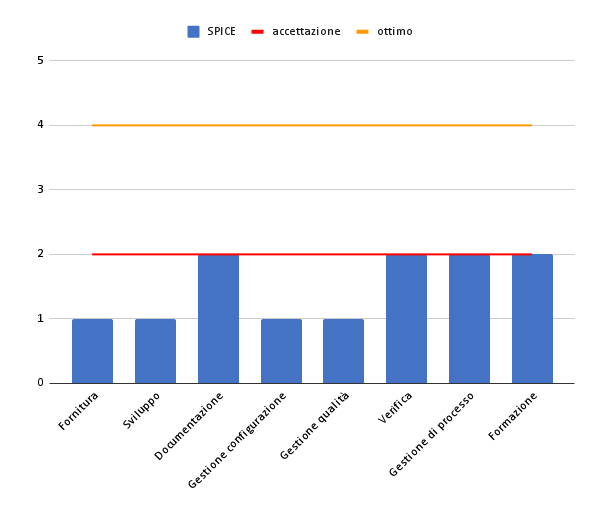
\includegraphics[scale=0.50]{Sezioni/images/analisi-spice.png}
    \caption{Analisi: MPC01 - SPICE}
\end{figure}

Alcune note sui risultati:
\begin{itemize}
\item I processi di Fornitura e Sviluppo non superano il livello 1 in quanto entrambi da considerarsi non totalmente controllati;
\item Il processo di Documentazione raggiunge il livello 2, il processo viene sottoposto a controllo e verifica, debole è l'aderenza agli standard e si stanno facendo dei passi avanti per renderlo ripetibile;
\item I processi di Gestione della configurazione e Gestione della qualità non essendo sottoposti a controlli ricadono nel livello 1, ma, almeno per la gestione della configurazione, le performance sono considerate ad un livello discreto e di conseguenza gli attributi intermedi vengono avanzati;
\item I processi di Verifica, Gestione di processo e Formazione, essendo ben istanziati e controllati, raggiungono il livello 2. 
\end{itemize}


\subsubsection{MPC02 - BCWS}
\begin{figure}[H]
    \centering
    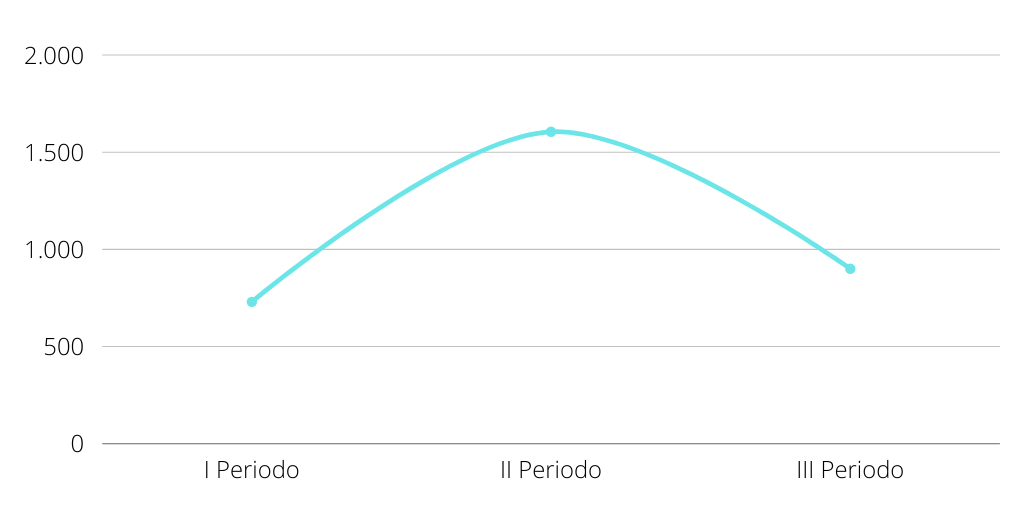
\includegraphics[scale=0.50]{Sezioni/images/analisi-bcws.png}
    \caption{Analisi: MPC02 - BCWS}
\end{figure}

\subsubsection{MPC03 - ACWP}
\begin{figure}[H]
    \centering
    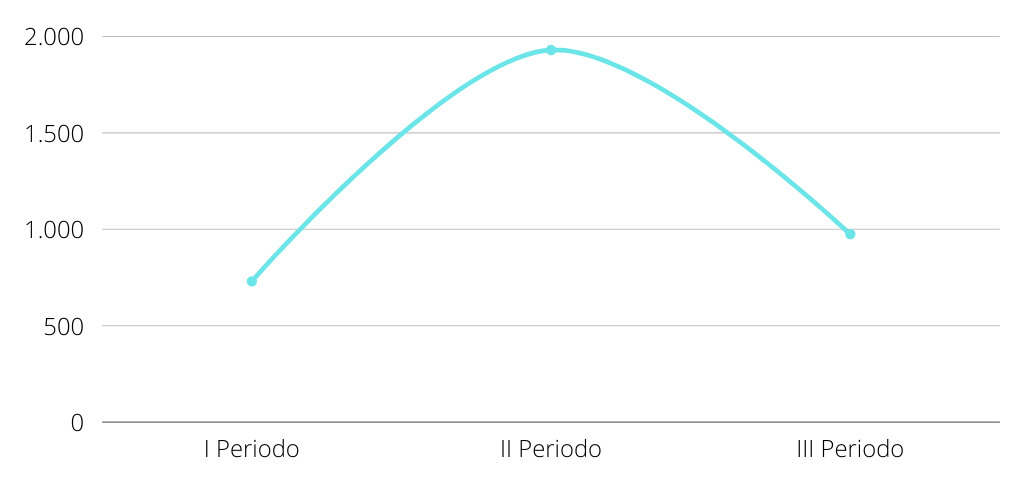
\includegraphics[scale=0.50]{Sezioni/images/analisi-acwp.png}
    \caption{Analisi: MPC02 - ACWP}
\end{figure}

\subsubsection{MPC04 - BCWP}
\begin{figure}[H]
    \centering
    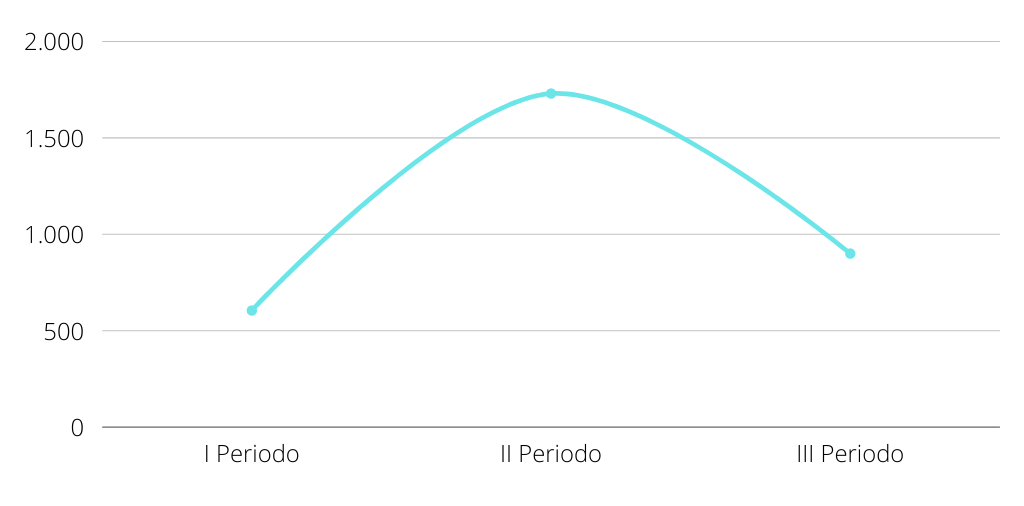
\includegraphics[scale=0.50]{Sezioni/images/analisi-BCWP.png}
    \caption{Analisi: MPC04 - BCWP}
\end{figure}


\subsubsection{MPC05 - Schedule variance}
Nel primo periodo il BCWP è inferiore al BCWS a causa di un errore nell'attività di analisi, il costo è stato recuperato nel periodo successivo.
\begin{figure}[H]
    \centering
    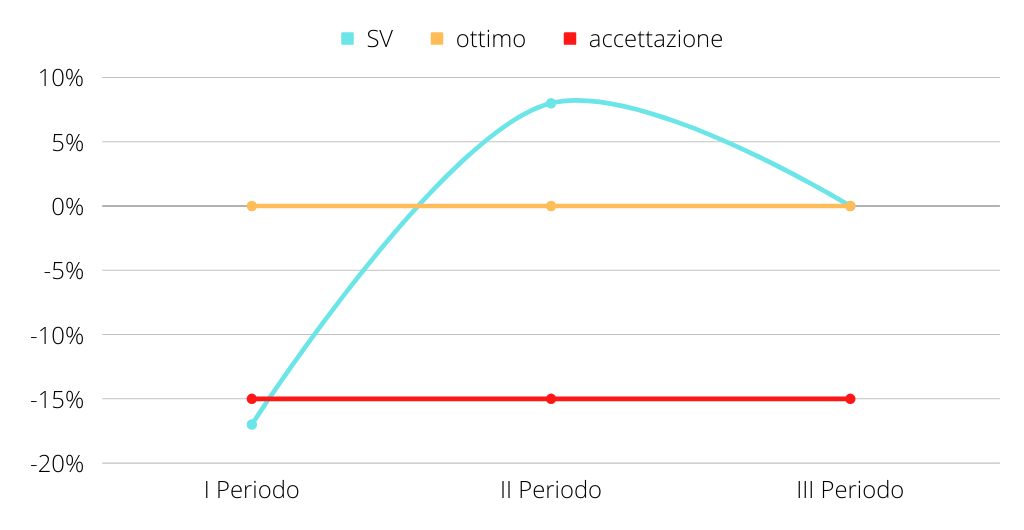
\includegraphics[scale=0.50]{Sezioni/images/analisi-SV.png}
    \caption{Analisi: MPC05 - SV}
\end{figure}

\subsubsection{MPC06 - Budget variance}
A causa dell'errore commesso durante il primo periodo nello svolgimento dell'attività di analisi, sono state necessarie più ore lavorative rispetto a quelle preventivate nel secondo periodo.
\begin{figure}[H]
    \centering
    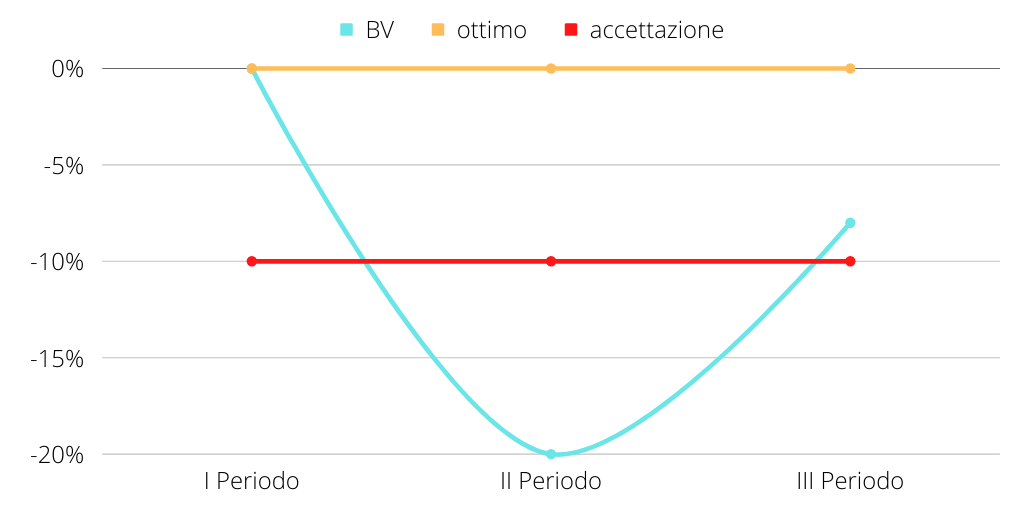
\includegraphics[scale=0.50]{Sezioni/images/analisi-BV.png}
    \caption{Analisi: MPC06 - BV}
\end{figure}

\subsubsection{MQP01 - Indice di Gulpease}
È stato calcolato l'indice di Gulpease di ogni documento redatto escludendo intestazione, registro delle modifiche e dati presenti nelle tabelle al fine di evitare risultati inesatti.
\begin{table}[H]
    \rowcolors{2}{gray!25}{white}
    \rowcolors{2}{gray!25}{white}
        \renewcommand{\arraystretch}{1.5}
        \begin{tabular}{m{0.4\textwidth}<{\centering}  m{0.25\textwidth}<{\centering}  m{0.25\textwidth}<{\centering} }
            \rowcolor{darkblue}
            \textcolor{white}{\textbf{Documento}}& \textcolor{white}{\textbf{Valore}} & \textcolor{white}{\textbf{Esito}}\\ 
            
			\textit{NormeDiProgetto-v0.2.0} &
            59 &
            Superato \\

            \textit{PianoDiProgetto-v0.3.0} &
            71 &
            Superato \\

            \textit{PianoDiQualifica-v0.1.0} &
            61 &
            Superato \\

            \textit{AnalisiDeiRequisiti-v0.3.0} &
            85 &
            Superato \\

            \textit{VerbaleInterno-2021.11.22}&
            75 &
            Superato \\

            \textit{VerbaleInterno-2021.11.29}&
            75 &
            Superato \\
            
            \textit{VerbaleInterno-2021.12.06}&
            64 &
            Superato \\
            
            \textit{VerbaleInterno-2021.12.13}&
            61 &
            Superato \\
            
            \textit{VerbaleInterno-2021.12.20}&
            77 &
            Superato \\
            
            \textit{VerbaleInterno-2021.12.29}&
            76 &
            Superato \\
            
            \textit{VerbaleInterno-2022.01.03}&
            77 &
            Superato \\
            
            \textit{VerbaleInterno-2022.01.07}&
            66 &
            Superato \\
            
            \textit{VerbaleInterno-2022.01.09}&
            88 &
            Superato \\
            
            \textit{VerbaleInterno-2022.01.13}&
            76 &
            Superato \\
            
            \textit{VerbaleInterno-2022.01.20}&
            65 &
            Superato \\

            \textit{VerbaleEsterno-2021.12.22}&
            75&
            Superato \\
            
    
    \end{tabular}
    \caption{Analisi: MQP01 - Indice di Gulpease}

	\begin{figure}[H]
        \centering
        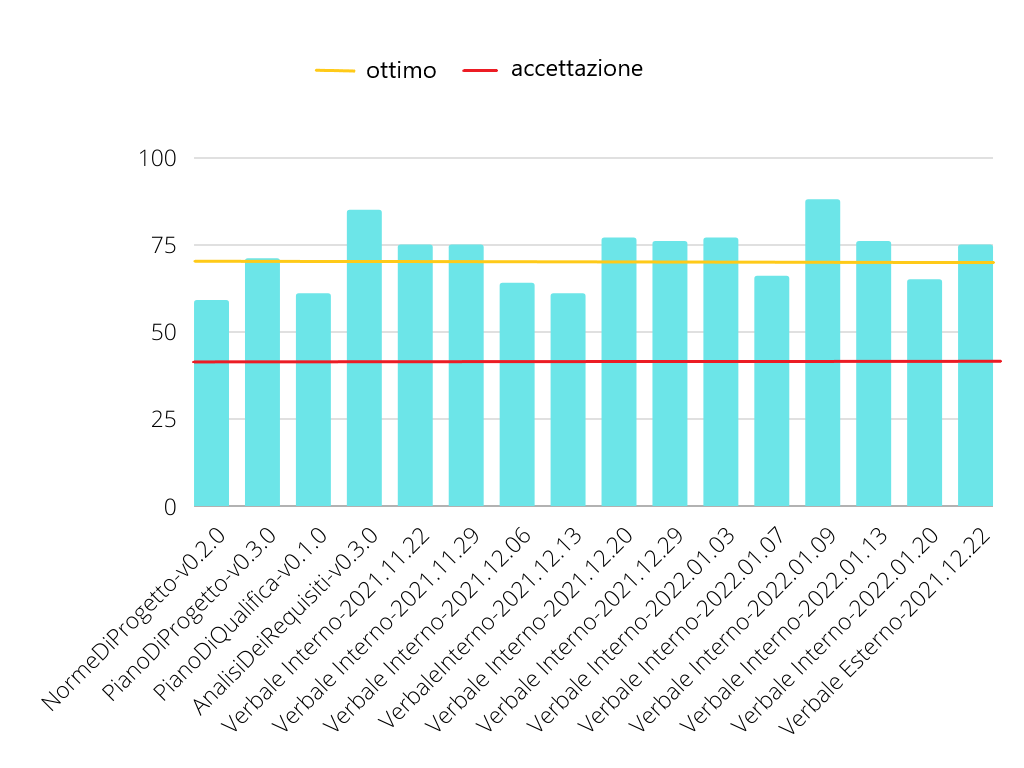
\includegraphics[scale=0.50]{Sezioni/images/analisi-gulpease.png}
        \caption{Analisi: MQP01 - Indice di Gulpease}
    \end{figure}
\end{table}

\subsection{Periodo di produzione del Proof of Concept}
In questo periodo vengono calcolate le metriche MPC01, MPC02, MPC03, MPC04, MPC05, MPC06, MPC07 e MQP01. Le restanti metriche non vengono calcolate perché nonostante sia stato prodotto del codice, lo è stato fatto in piccola parte.
\subsubsection{MPC01 - SPICE}
Ogni sigla presente in questa sezione fa riferimento a quanto descritto all'interno del documento \textit{\NdP} §A


\begin{table}[H]
    \rowcolors{2}{gray!25}{white}
    \rowcolors{2}{gray!25}{white}
        \renewcommand{\arraystretch}{1.5}
        \begin{tabular}{ m{0.15\textwidth}<{\centering}  m{0.055\textwidth}<{\centering} m{0.055\textwidth}<{\centering} m{0.055\textwidth}<{\centering} m{0.055\textwidth}<{\centering} m{0.055\textwidth}<{\centering} m{0.055\textwidth}<{\centering} m{0.055\textwidth}<{\centering} m{0.055\textwidth}<{\centering} m{0.055\textwidth}<{\centering} m{0.08\textwidth}<{\centering}}
	\rowcolor{darkblue}
	\textcolor{white}{\textbf{Processo}} &\textcolor{white}{\textbf{1.1}} &\textcolor{white}{\textbf{2.1}} &\textcolor{white}{\textbf{2.2}} &\textcolor{white}{\textbf{3.1}} &\textcolor{white}{\textbf{3.2}} &\textcolor{white}{\textbf{4.1}} &\textcolor{white}{\textbf{4.2}} &\textcolor{white}{\textbf{5.1}} &\textcolor{white}{\textbf{5.2}} &\textcolor{white}{\textbf{Livello}}\\ 


	Fornitura & F & L & L & N & N & N & N & N & N & 1 \\
    Sviluppo & F & L & L & N & N & N & N & N & N & 1 \\
    Documentazione & F & F & F & L & L & N & N & N & N & 2 \\
    Gestione della configurazione & F & F & F & N & N & N & N & N & N & 2 \\
    Gestione della qualità & F & F & F & N & N & N & N & N & N & 2 \\
    Verifica & F & F & F & P & P & N & N & N & N & 2 \\
   Validazione & F & P & P & N & N & N & N & N & N & 1 \\
    Gestione di processo & F & F & F & N & N & N & N & N & N & 2 \\
    Formazione dei membri del team & F & F & F & N & N & N & N & N & N & 2 \\
    
\end{tabular}       
\caption{Produzione del Proof of Concept: MPC01 - SPICE}
\end{table}

\begin{figure}[H]
    \centering
    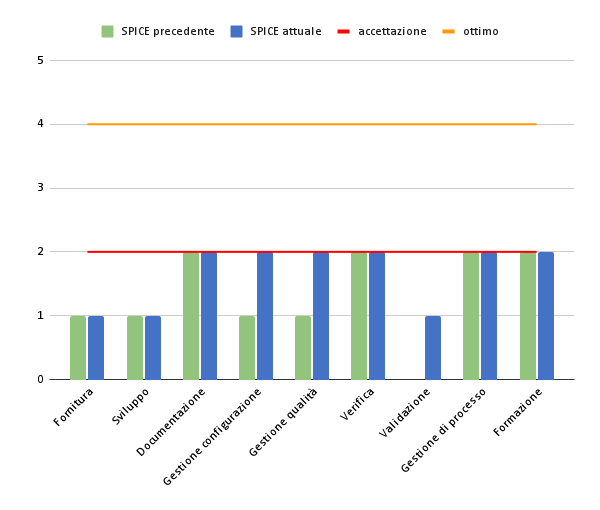
\includegraphics[scale=0.50]{Sezioni/images/poc-spice.png}
    \caption{Produzione del Proof of Concept: MPC01 - SPICE}
\end{figure}

   Alcune note sui risultati:
\begin{itemize}
\item I processi di Fornitura e Sviluppo restano al livello 1 ma la copertura degli attributi interni è migliorata;
\item Il processo di Documentazione resta al livello 2, ma c'è un miglioramento in relazione al rispetto delle norme e standard e il processo è a pochi passi da essere considerato ripetibile;
\item I processi di Gestione della configurazione e Gestione della qualità raggiungono il livello 2, in quanto sono stati rivisti e migliorati poiché sono diventanti più prominenti nella fase corrente;
\item I processi di Verifica, Gestione di processo e Formazione, restano al livello 2, non sono stati identificati cambiamenti di nota tranne per il processo di Verifica, in quanto è stato iniziato un lavoro di standardizzazione; 
\item Viene istanziato il nuovo processo di Validazione, non supera il livello 1 (in quando non è pienamente controllato), ma si punta ad un miglioramento delle performance.
\end{itemize}   


\subsubsection{MPC02 - BCWS}
\begin{figure}[H]
    \centering
    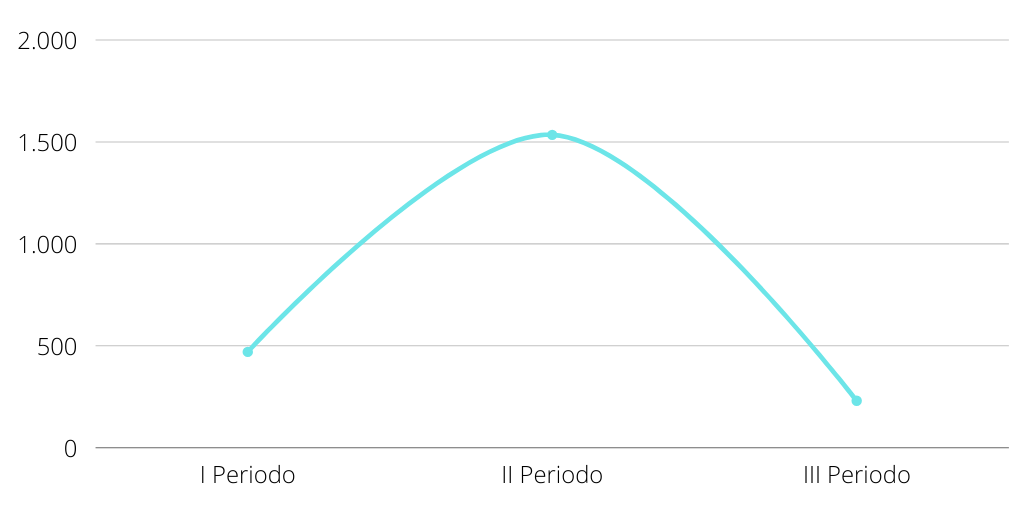
\includegraphics[scale=0.50]{Sezioni/images/poc-bcws.png}
    \caption{Produzione del Proof of Concept: MPC02 - BCWS}
\end{figure}

\subsubsection{MPC03 - ACWP}
\begin{figure}[H]
    \centering
    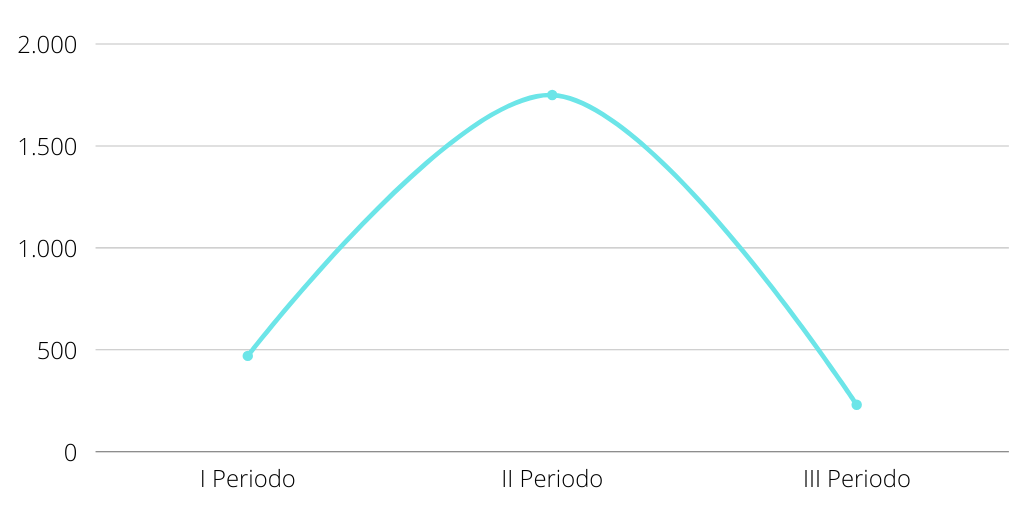
\includegraphics[scale=0.50]{Sezioni/images/poc-acwp.png}
    \caption{Produzione del Proof of Concept: MPC03 - ACWP}
\end{figure}

\subsubsection{MPC04 - BCWP}
\begin{figure}[H]
    \centering
    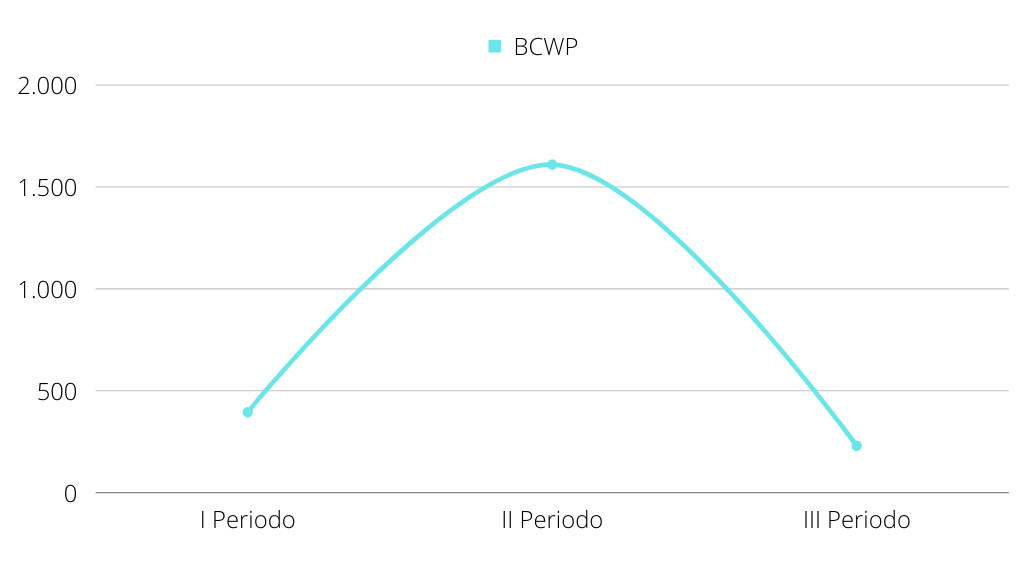
\includegraphics[scale=0.50]{Sezioni/images/poc-BCWP.png}
    \caption{Produzione del Proof of Concept: MPC04 - BCWP}
\end{figure}

\subsubsection{MPC05 - Schedule variance}
Nel primo periodo il BCWP è inferiore al BCWS a causa di un incomprensione per la realizzazione del Proof of Concept, il costo in questione è stato recuperato nel periodo successivo.
\begin{figure}[H]
    \centering
    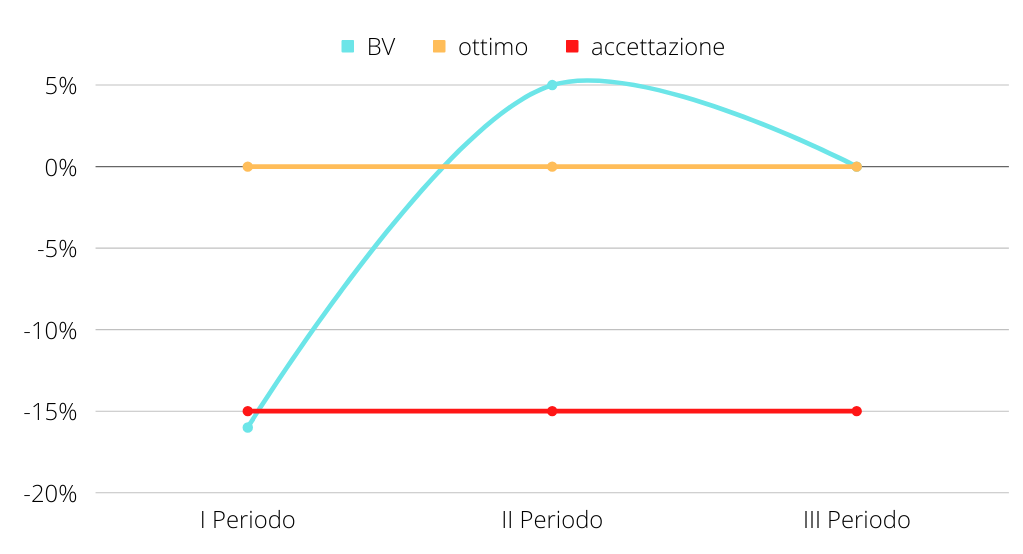
\includegraphics[scale=0.50]{Sezioni/images/poc-SV.png}
    \caption{Produzione del Proof of Concept: MPC05 - SV}
\end{figure}

\subsubsection{MPC06 - Budget variance}
A causa dell'incomprensione sulla realizzazione del Proof of Concept avvenuta nel primo periodo, è stato necessario impiegare più ore lavorative rispetto a quelle preventivate nel secondo periodo.
\begin{figure}[H]
    \centering
    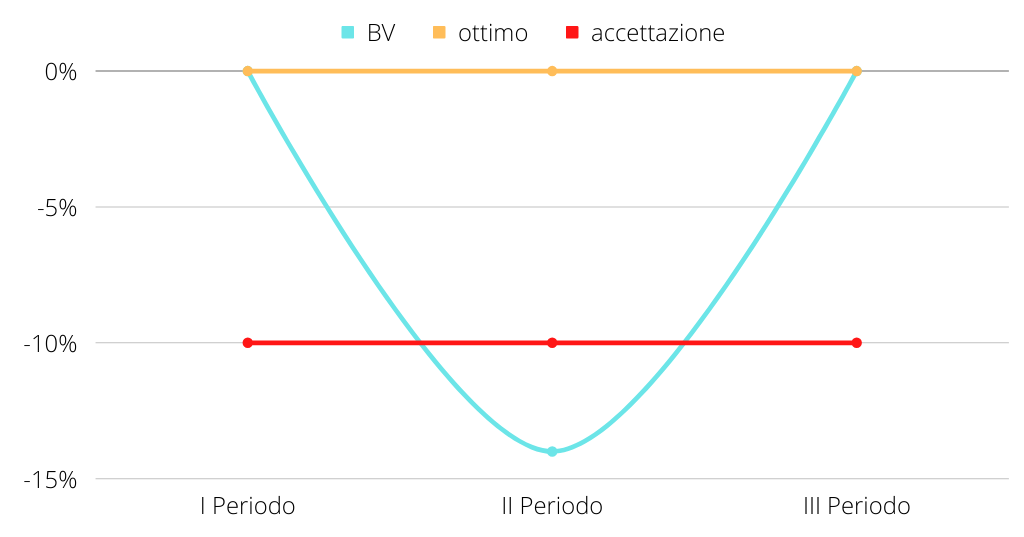
\includegraphics[scale=0.50]{Sezioni/images/poc-BV.png}
    \caption{Produzione del Proof of Concept: MPC06 - BV}
\end{figure}

\subsubsection{MQP01 - Indice di Gulpease}
È stato calcolato l'indice di Gulpease di ogni documento redatto escludendo intestazione, registro delle modifiche e dati presenti nelle tabelle al fine di evitare risultati inesatti.
\begin{table}[H]
    \rowcolors{2}{gray!25}{white}
    \rowcolors{2}{gray!25}{white}
        \renewcommand{\arraystretch}{1.5}
        \begin{tabular}{m{0.4\textwidth}<{\centering}  m{0.25\textwidth}<{\centering}  m{0.25\textwidth}<{\centering} }
            \rowcolor{darkblue}
            \textcolor{white}{\textbf{Documento}}& \textcolor{white}{\textbf{Valore}} & \textcolor{white}{\textbf{Esito}}\\ 

            \textit{NormeDiProgetto-v1.0.0} &
            75 &
            Superato \\

            \textit{PianoDiProgetto-v1.0.0} &
            69 &
            Superato \\

            \textit{PianoDiQualifica-v1.0.0} &
            59 &
            Superato \\

            \textit{AnalisiDeiRequisiti-v1.0.0} &
            84 &
            Superato \\
            
            \textit{Glossario-v1.0.0} &
            73 &
            Superato \\

            \textit{VerbaleInterno-2022.01.27} &
            60 &
            Superato \\
            
            \textit{VerbaleInterno-2022.02.03} &
            60 &
            Superato \\

            \textit{VerbaleEsterno-2022.01.26} &
            57&
            Superato \\

            \textit{VerbaleEsterno-2022.02.08} &
            61&
            Superato \\
    \end{tabular}
    \caption{Produzione del Proof of Concept: MQP01 - Indice di Gulpease}
\end{table}

\begin{figure}[H]
    \centering
    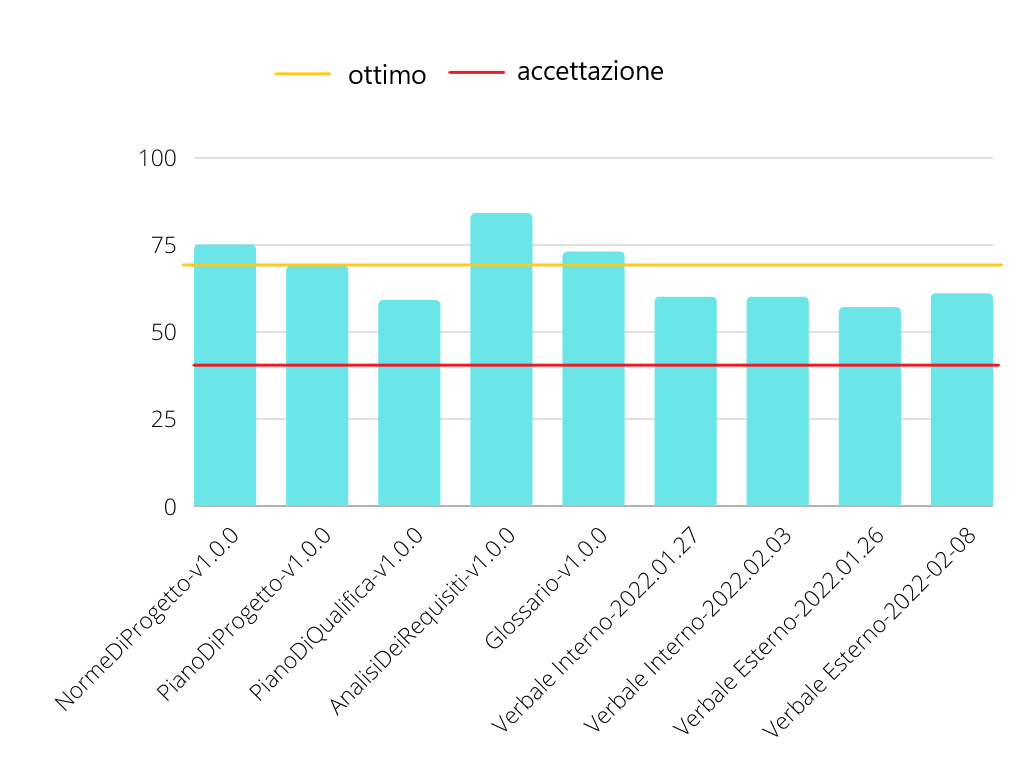
\includegraphics[scale=0.50]{Sezioni/images/poc-gulpease.png}
    \caption{Produzione del Proof of Concept: MQP01 - Indice di Gulpease}
\end{figure}

Segue l'andamento dell'indice di Gulpease per i documenti:
\begin{itemize}
    \item \textit{NormeDiProgetto-v1.0.0};
    \item \textit{PianoDiProgetto-v1.0.0};
    \item \textit{AnalisiDeiRequisiti-v1.0.0};
    \item \textit{PianoDiQualifica-v1.0.0}.
\end{itemize}

\begin{figure}[H]
    \centering
    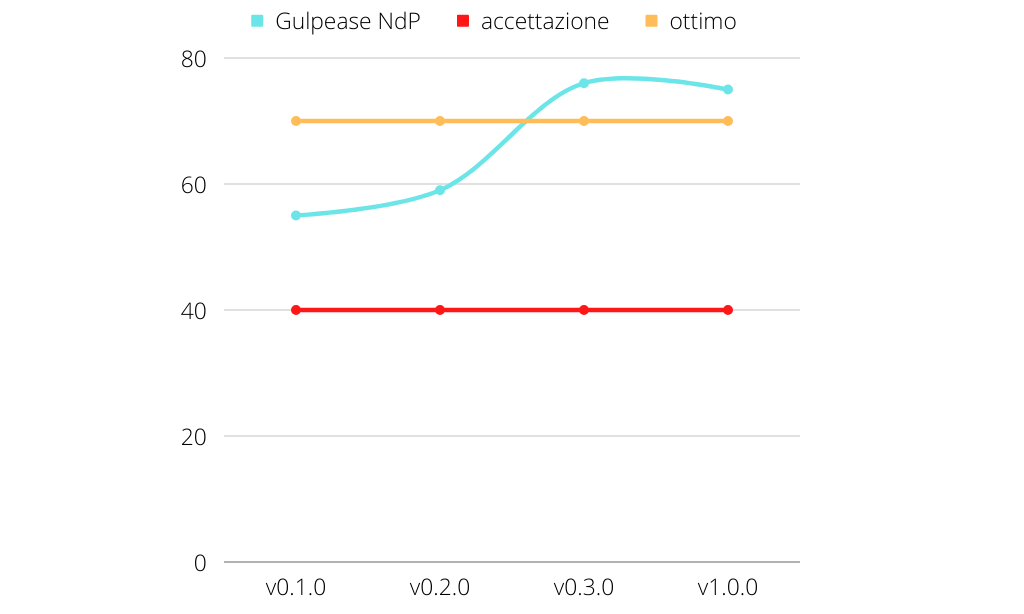
\includegraphics[scale=0.50]{Sezioni/images/poc-gulpease-ndp.png}
    \caption{Produzione del Proof of Concept: MQP01 - NdP}
\end{figure}


\begin{figure}[H]
    \centering
    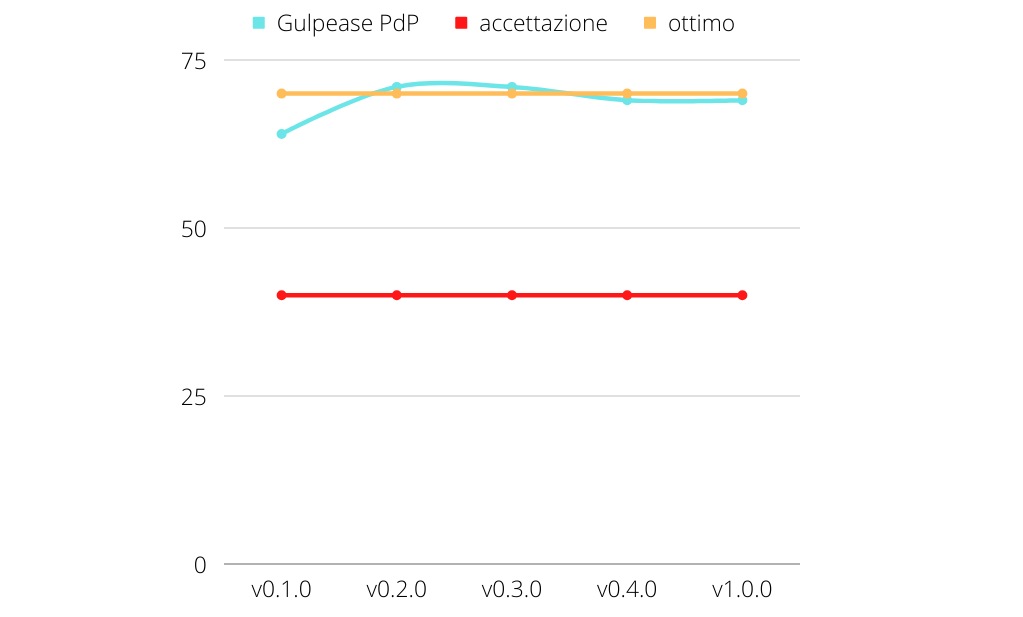
\includegraphics[scale=0.50]{Sezioni/images/poc-gulpease-pdp.png}
    \caption{Produzione del Proof of Concept: MQP01 - PdP}
\end{figure}


\begin{figure}[H]
    \centering
    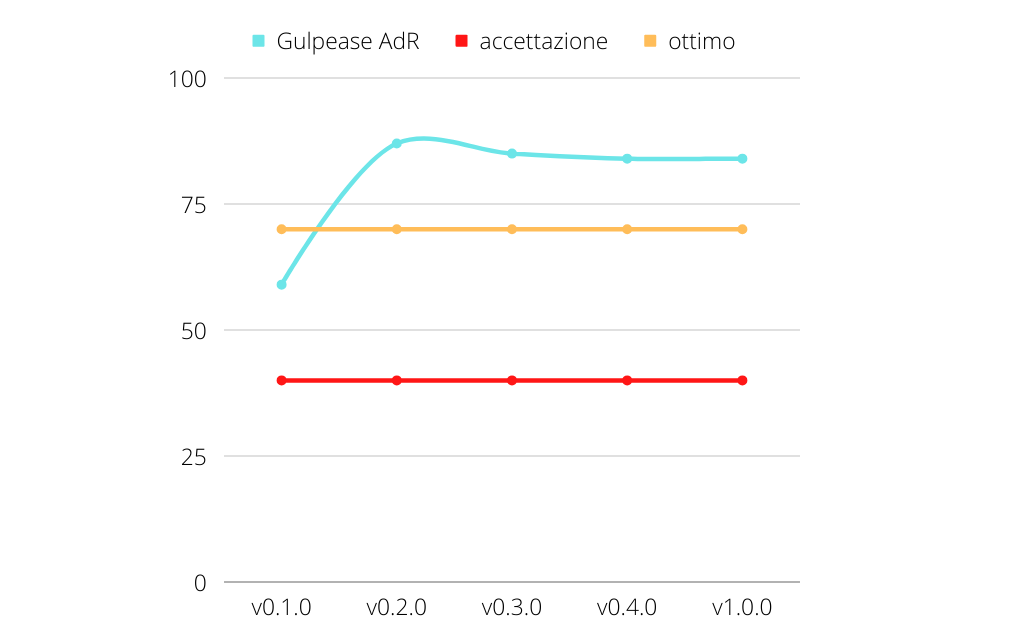
\includegraphics[scale=0.50]{Sezioni/images/poc-gulpease-adr.png}
    \caption{Produzione del Proof of Concept: MQP01 - AdR}
\end{figure}


\begin{figure}[H]
    \centering
    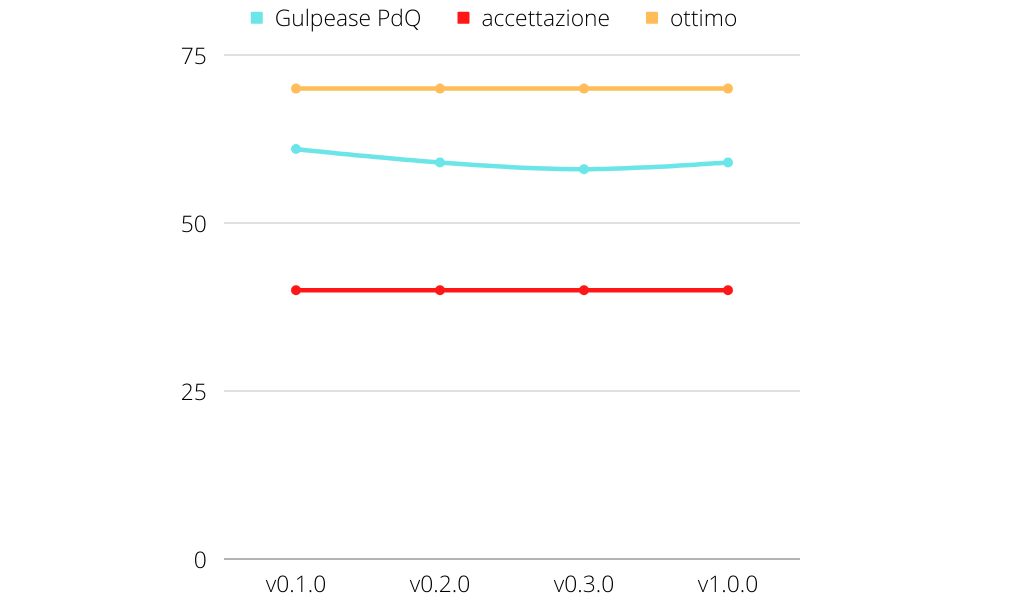
\includegraphics[scale=0.50]{Sezioni/images/poc-gulpease-pdq.png}
    \caption{Produzione del Proof of Concept: MQP01 - PdQ}
\end{figure}

\pagebreak
\subsection{Periodo di Progettazione di dettaglio e codifica}
\subsubsection{MPC01 - SPICE}
Ogni sigla presente in questa sezione fa riferimento a quanto descritto all'interno del documento \textit{NormeDiProgetto-v2.0.0} §A


\begin{table}[H]
    \rowcolors{2}{gray!25}{white}
    \rowcolors{2}{gray!25}{white}
        \renewcommand{\arraystretch}{1.5}
        \begin{tabular}{ m{0.15\textwidth}<{\centering}  m{0.055\textwidth}<{\centering} m{0.055\textwidth}<{\centering} m{0.055\textwidth}<{\centering} m{0.055\textwidth}<{\centering} m{0.055\textwidth}<{\centering} m{0.055\textwidth}<{\centering} m{0.055\textwidth}<{\centering} m{0.055\textwidth}<{\centering} m{0.055\textwidth}<{\centering} m{0.08\textwidth}<{\centering}}
	\rowcolor{darkblue}
	\textcolor{white}{\textbf{Processo}} &\textcolor{white}{\textbf{1.1}} &\textcolor{white}{\textbf{2.1}} &\textcolor{white}{\textbf{2.2}} &\textcolor{white}{\textbf{3.1}} &\textcolor{white}{\textbf{3.2}} &\textcolor{white}{\textbf{4.1}} &\textcolor{white}{\textbf{4.2}} &\textcolor{white}{\textbf{5.1}} &\textcolor{white}{\textbf{5.2}} &\textcolor{white}{\textbf{Livello}}\\ 


    Fornitura & F & F & F & P & L & N & N & N & N & 2 \\
    Sviluppo & F & F & F & F & F & N & N & N & N & 3 \\
    Documentazione & F & F & F & L & L & N & N & N & N & 2 \\
    Gestione della configurazione & F & F & F & N & N & N & N & N & N & 2 \\
    Gestione della qualità & F & F & F & F & F & N & N & N & N & 3 \\
    Verifica & F & F & F & L & P & N & N & N & N & 2 \\
   
    Gestione di processo & F & F & F & P & P & N & N & N & N & 2 \\
    Formazione dei membri del team & F & F & F & N & N & N & N & N & N & 2 \\
    
\end{tabular}       
\caption{Progettazione di dettaglio e codifica: MPC01 - SPICE}
\end{table}

\begin{figure}[H]
    \centering
    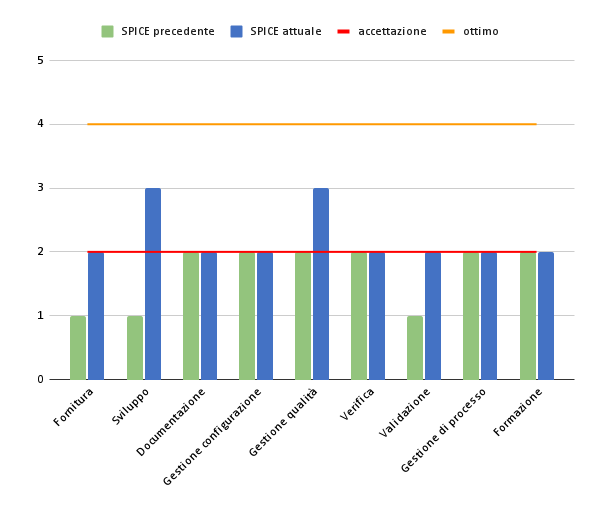
\includegraphics[scale=0.50]{Sezioni/images/pdc-spice.png}
    \caption{Progettazione di dettaglio e codifica: MPC01 - SPICE}
\end{figure}

   Alcune note sui risultati:
\begin{itemize}
\item Il processo di sviluppo passa dal livello 1 al livello 3
\item Il processo di gestione della qualità sale al livello 3
\item I processi di Fornitura e Validazione salgono al livello 2 raggiungendo così il valore tollerato
\item I restanti processi rimangono al livello 2, tuttavia buona parte di loro sono migliorati rispetto al periodo precedente ed è ragionevole pensare di raggiungere il livello 3 in futuro.
\end{itemize}


\subsubsection{MPC02 - BCWS}
\begin{figure}[H]
    \centering
    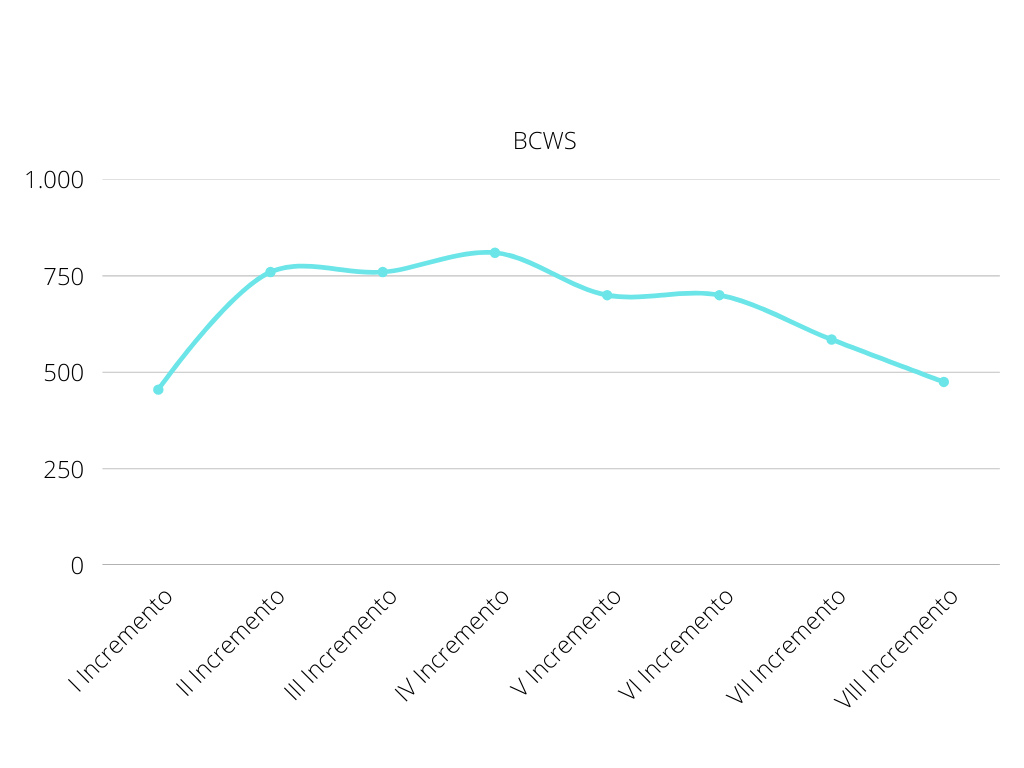
\includegraphics[scale=0.50]{Sezioni/images/pdc-BCWS.png}
    \caption{Progettazione di dettaglio e codifica: MPC02 - BCWS}
\end{figure}

\subsubsection{MPC03 - ACWP}
\begin{figure}[H]
    \centering
    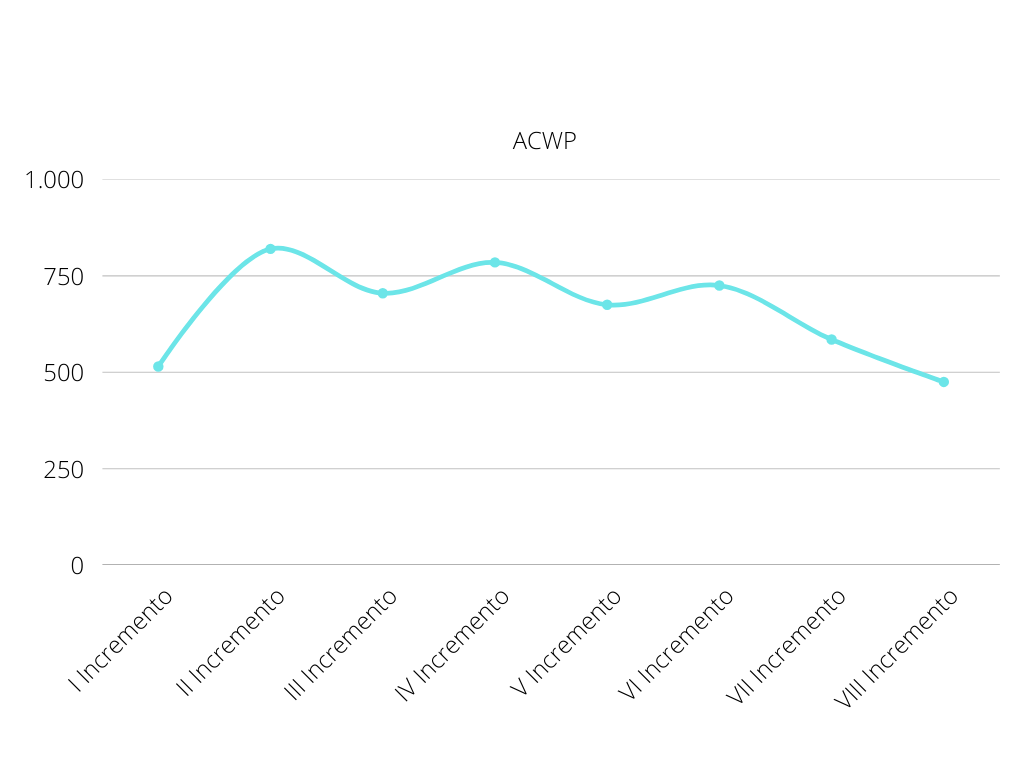
\includegraphics[scale=0.50]{Sezioni/images/pdc-ACWP.png}
    \caption{Progettazione di dettaglio e codifica: MPC03 - ACWP}
\end{figure}

\subsubsection{MPC04 - BCWP}
\begin{figure}[H]
    \centering
    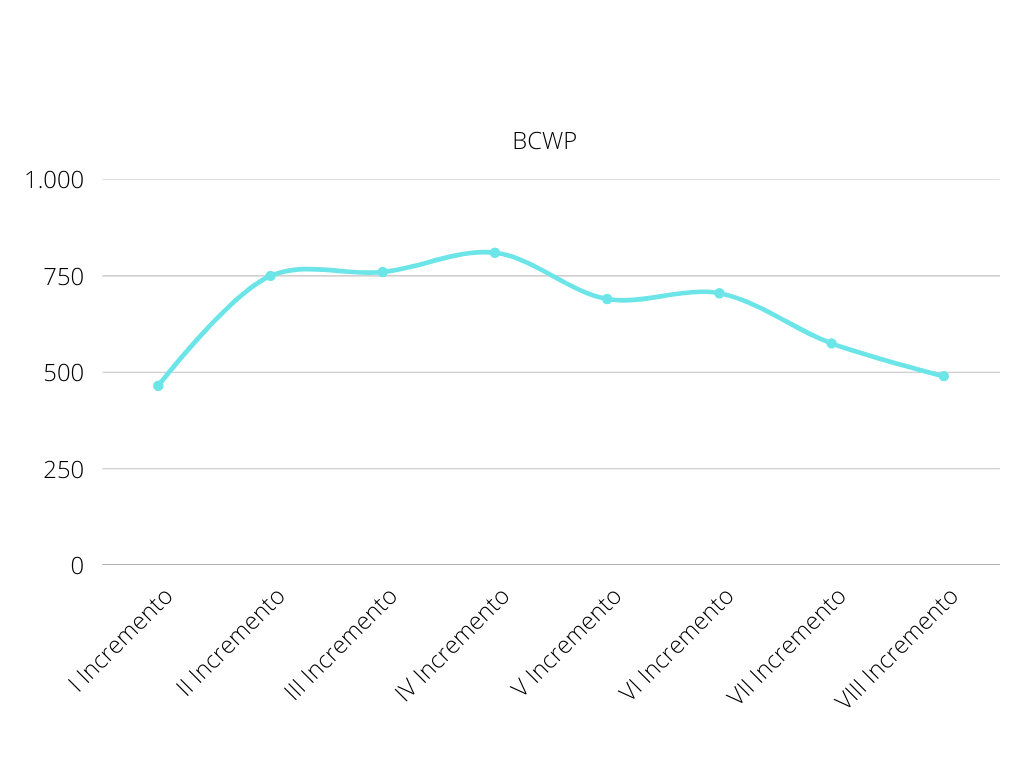
\includegraphics[scale=0.50]{Sezioni/images/pdc-BCWP.png}
    \caption{Progettazione di dettaglio e codifica: MPC04 - BCWP}
\end{figure}

\subsubsection{MPC05 - Schedule variance}
\begin{figure}[H]
    \centering
    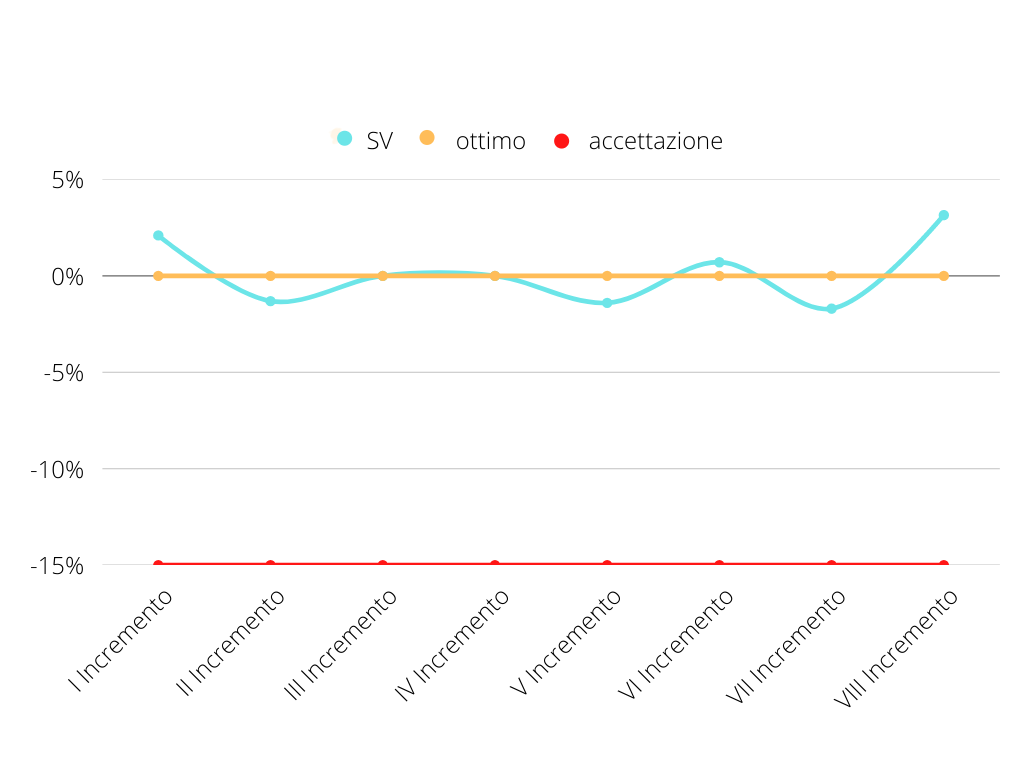
\includegraphics[scale=0.50]{Sezioni/images/pdc-SV.png}
    \caption{Progettazione di dettaglio e codifica: MPC05 - SV}
\end{figure}

\subsubsection{MPC06 - Budget variance}
\begin{figure}[H]
    \centering
    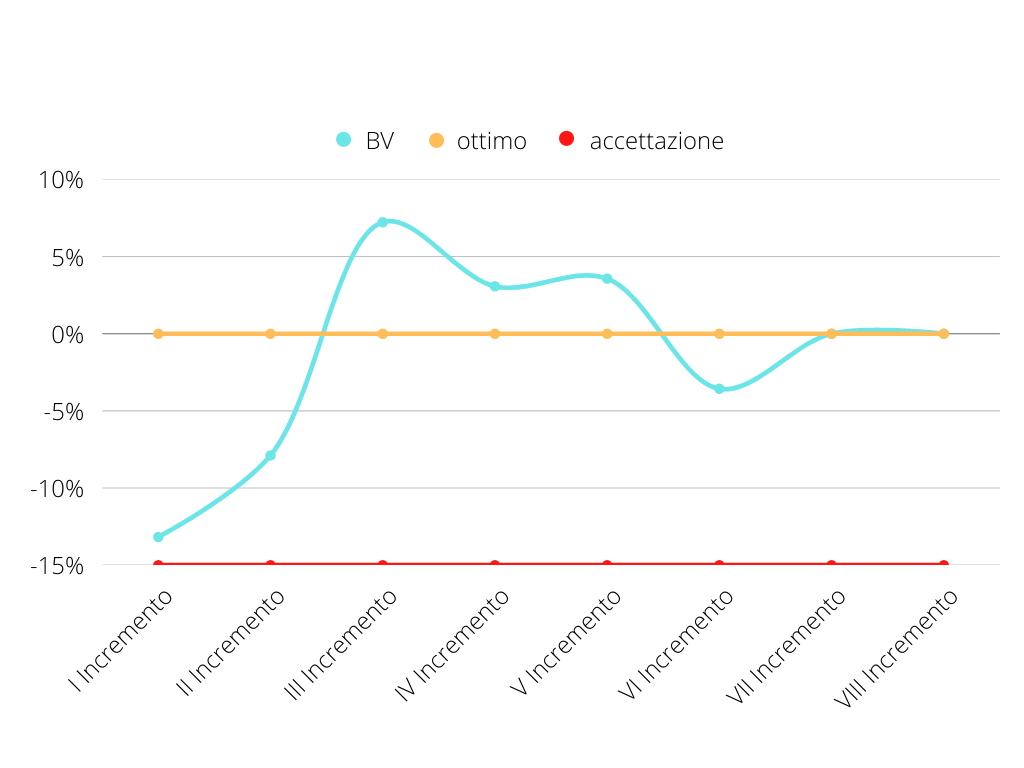
\includegraphics[scale=0.50]{Sezioni/images/pdc-BV.png}
    \caption{Progettazione di dettaglio e codifica: MPC06 - BV}
\end{figure}
\subsection{Periodo di Progettazione di dettaglio e codifica}
\subsubsection{MQP01 - Indice di Gulpease}
\begin{table}[H]
    \rowcolors{2}{gray!25}{white}
    \rowcolors{2}{gray!25}{white}
        \renewcommand{\arraystretch}{1.5}
        \begin{tabular}{m{0.4\textwidth}<{\centering}  m{0.25\textwidth}<{\centering}  m{0.25\textwidth}<{\centering} }
            \rowcolor{darkblue}
            \textcolor{white}{\textbf{Documento}}& \textcolor{white}{\textbf{Valore}} & \textcolor{white}{\textbf{Esito}}\\ 

            \textit{NormeDiProgetto-v2.0.0} &
            65 &
            Superato \\

            \textit{PianoDiProgetto-v2.0.0} &
            73 &
            Superato \\

            \textit{PianoDiQualifica-v2.0.0} &
            66 &
            Superato \\

            \textit{AnalisiDeiRequisiti-v2.0.0} &
            88 &
            Superato \\
            
            \textit{Glossario-v2.0.0} &
            80 &
            Superato \\

            \textit{VerbaleEsterno-2022.03.03} &
            70 &
            Superato \\
            
            \textit{VerbaleEsterno-2022.04.08} &
            70 &
            Superato \\

            \textit{VerbaleEsterno-2022.04.28} &
            78&
            Superato \\

            \textit{VerbaleInterno-2022.02.23} &
            79&
            Superato \\
            \textit{VerbaleInterno-2022.02.28} &
            72&
            Superato \\
            \textit{VerbaleInterno-2022.03.07} &
            70&
            Superato \\
            \textit{VerbaleInterno-2022.03.14} &
            70&
            Superato \\
            \textit{VerbaleInterno-2022.04.04} &
            75&
            Superato \\
            \textit{VerbaleInterno-2022.04.11} &
            76&
            Superato \\
            \textit{VerbaleInterno-2022.04.25} &
            77&
            Superato \\
            \textit{VerbaleInterno-2022.05.09} &
            73&
            Superato \\
    \end{tabular}
    \caption{Progettazione di dettaglio e codifica: MQP01 - Indice di Gulpease}
\end{table}
\begin{figure}[H]
    \centering
    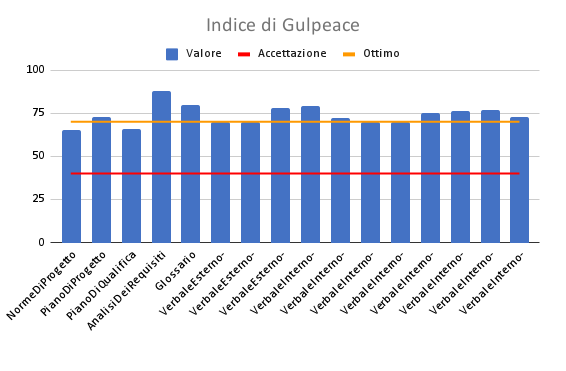
\includegraphics[scale=0.50]{Sezioni/images/pb prodotto/Indice di Gulpeace.png}
    \caption{Progettazione di dettaglio e codifica: MPC02 - BCWS}
\end{figure}
\subsubsection{MQP02 - Profondità di una gerarchia}
\begin{figure}[H]
    \centering
    \includegraphics[scale=0.50]{Sezioni/images/pb prodotto/Profondità di una gerarchia.png}
    \caption{Progettazione di dettaglio e codifica: MQP02 - Profondità di una gerarchia}
\end{figure}
\subsubsection{MQP03 - Numero parametri per metodo}
\begin{figure}[H]
    \centering
    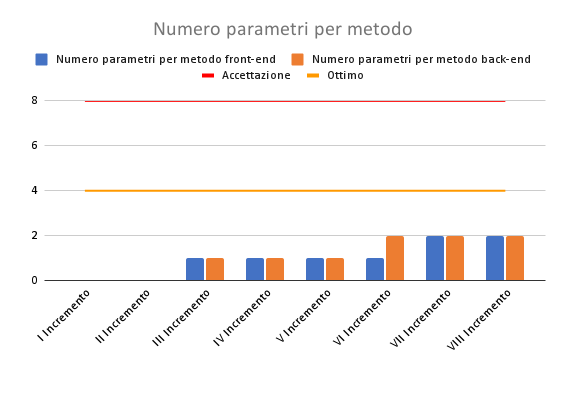
\includegraphics[scale=0.50]{Sezioni/images/pb prodotto/Numero parametri per metodo.png}
    \caption{Progettazione di dettaglio e codifica: MQP03 - Numero parametri per metodo}
\end{figure}
\subsubsection{MQP04 - Code coverage}
\begin{figure}[H]
    \centering
    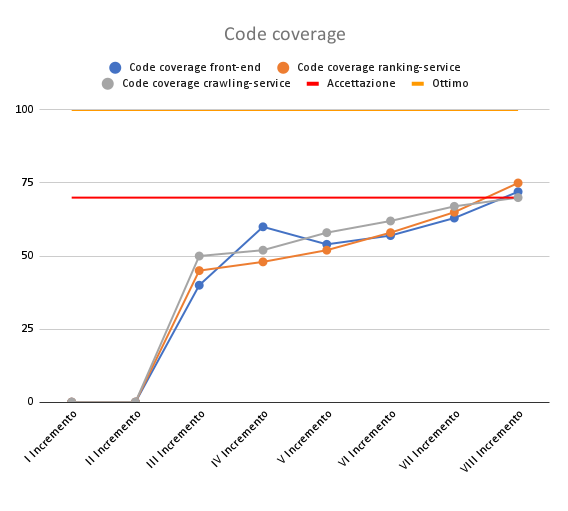
\includegraphics[scale=0.50]{Sezioni/images/pb prodotto/Code coverage.png}
    \caption{Progettazione di dettaglio e codifica: MQP04 - Code coverage}
\end{figure}
\subsubsection{MQP05 - Percentuale requisiti obbligatori soddisfatti}
\begin{figure}[H]
    \centering
    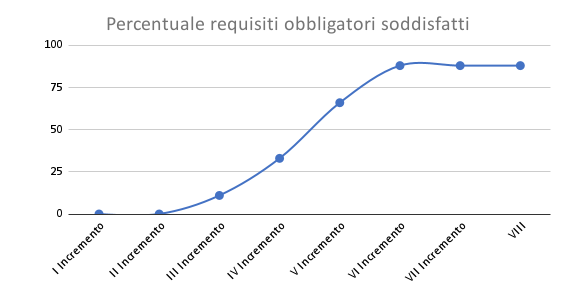
\includegraphics[scale=0.50]{Sezioni/images/pb prodotto/Percentuale requisiti obbligatori soddisfatti.png}
    \caption{Progettazione di dettaglio e codifica: MQP05 - Percentuale requisiti obbligatori soddisfatti}
\end{figure}
\subsubsection{MQP06 - Complessità ciclomatica}
\begin{figure}[H]
    \centering
    \includegraphics[scale=0.50]{Sezioni/images/pb prodotto/Complessità ciclomatica.png}
    \caption{Progettazione di dettaglio e codifica: MQP06 - Complessità ciclomatica}
\end{figure}
\subsubsection{MQP07 - Numero di bug}
\begin{figure}[H]
    \centering
    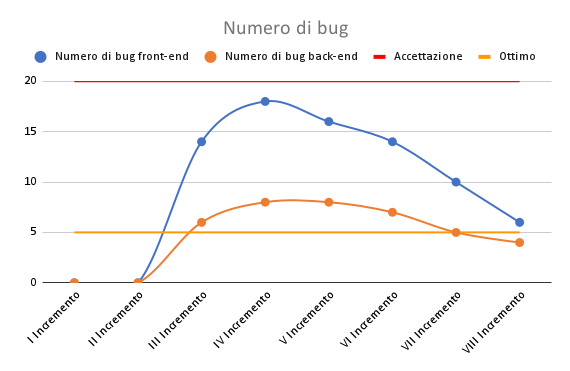
\includegraphics[scale=0.50]{Sezioni/images/pb prodotto/Numero di bug.png}
    \caption{Progettazione di dettaglio e codifica: MQP07 - Numero di bug}
\end{figure}
\subsubsection{MQP08 - Numero di Code smell}
\begin{figure}[H]
    \centering
    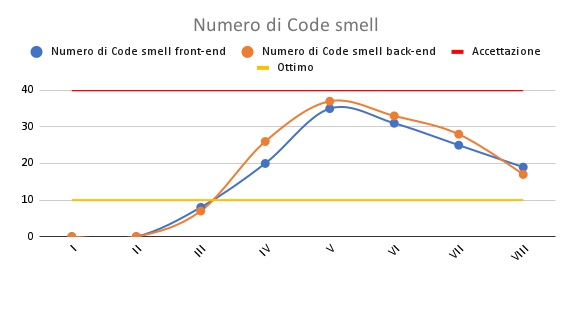
\includegraphics[scale=0.50]{Sezioni/images/pb prodotto/Numero di Code smell.png}
    \caption{Progettazione di dettaglio e codifica: MQP08 - Numero di Code smell}
\end{figure}
\subsubsection{MQP09 - Linee di Commento per Linee di Codice}
\begin{figure}[H]
    \centering
    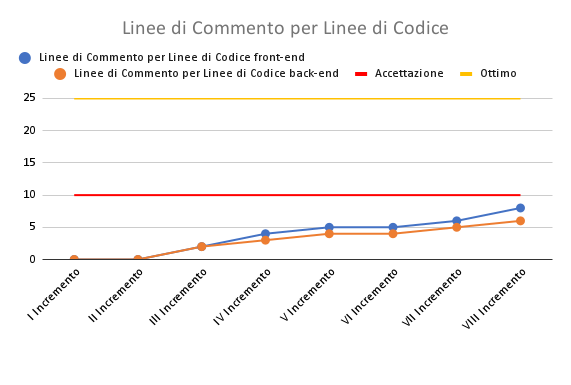
\includegraphics[scale=0.50]{Sezioni/images/pb prodotto/Linee di Commento per Linee di Codice.png}
    \caption{Progettazione di dettaglio e codifica: MQP09 - Linee di Commento per Linee di Codice}
\end{figure}
\subsubsection{MQP10 - Branch Coverage}
\begin{figure}[H]
    \centering
    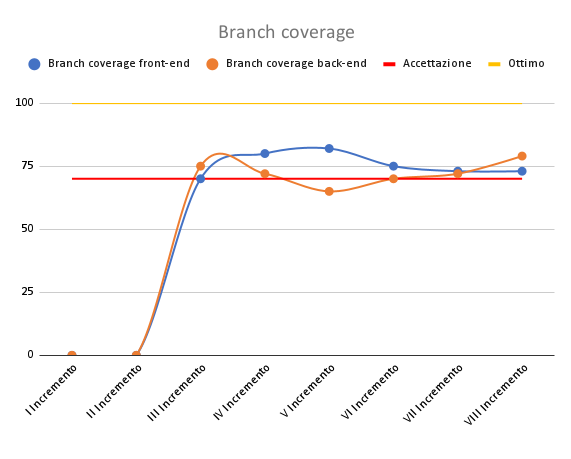
\includegraphics[scale=0.50]{Sezioni/images/pb prodotto/Branch coverage .png}
    \caption{Progettazione di dettaglio e codifica: MQP10 - Branch Coverage}
\end{figure}
\subsubsection{MQP11 - Successo di test}
\begin{figure}[H]
    \centering
    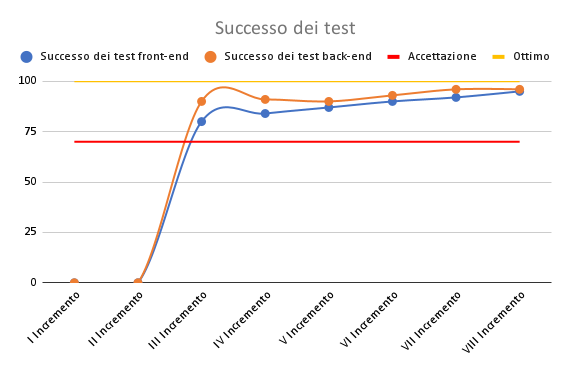
\includegraphics[scale=0.50]{Sezioni/images/pb prodotto/Successo dei test.png}
    \caption{Progettazione di dettaglio e codifica: MQP11 - Successo di test}
\end{figure}
\subsubsection{MQP12 - Numero di vulnerabilità}
\begin{figure}[H]
    \centering
    \includegraphics[scale=0.50]{Sezioni/images/pb prodotto/Numero di vulnerabilità.png}
    \caption{Progettazione di dettaglio e codifica: MQP12 - Numero di vulnerabilità}
\end{figure}

\subsection{Periodo di Validazione e collaudo}
\subsubsection{MPC01 - SPICE}
Ogni sigla presente in questa sezione fa riferimento a quanto descritto all'interno del documento \textit{NormeDiProgetto-v3.0.0} §A\newline \newline
Data la brevità del periodo, gli unici processi che salgono di livello sono quelli di fornitura e gestione della configurazione. Nonostante questo tutti i processi raggiungono la soglia di accettazione.


\begin{table}[H]
    \rowcolors{2}{gray!25}{white}
    \rowcolors{2}{gray!25}{white}
        \renewcommand{\arraystretch}{1.5}
        \begin{tabular}{ m{0.15\textwidth}<{\centering}  m{0.055\textwidth}<{\centering} m{0.055\textwidth}<{\centering} m{0.055\textwidth}<{\centering} m{0.055\textwidth}<{\centering} m{0.055\textwidth}<{\centering} m{0.055\textwidth}<{\centering} m{0.055\textwidth}<{\centering} m{0.055\textwidth}<{\centering} m{0.055\textwidth}<{\centering} m{0.08\textwidth}<{\centering}}
	\rowcolor{darkblue}
	\textcolor{white}{\textbf{Processo}} &\textcolor{white}{\textbf{1.1}} &\textcolor{white}{\textbf{2.1}} &\textcolor{white}{\textbf{2.2}} &\textcolor{white}{\textbf{3.1}} &\textcolor{white}{\textbf{3.2}} &\textcolor{white}{\textbf{4.1}} &\textcolor{white}{\textbf{4.2}} &\textcolor{white}{\textbf{5.1}} &\textcolor{white}{\textbf{5.2}} &\textcolor{white}{\textbf{Livello}}\\ 


    Fornitura & F & F & F & F & F & N & N & N & N & 3 \\
    Sviluppo & F & F & F & F & F & N & N & N & N & 3 \\
    Documentazione & F & F & F & L & L & N & N & N & N & 2 \\
    Gestione della configurazione & F & F & F & F & F & N & N & N & N & 3 \\
    Gestione della qualità & F & F & F & F & F & N & N & N & N & 3 \\
    Verifica & F & F & F & L & P & N & N & N & N & 2 \\
   
    Gestione di processo & F & F & F & P & P & N & N & N & N & 2 \\
    Formazione dei membri del team & F & F & F & N & N & N & N & N & N & 2 \\
    
\end{tabular}       
\caption{Validazione e collaudo: MPC01 - SPICE}
\end{table}

\begin{figure}[H]
    \centering
    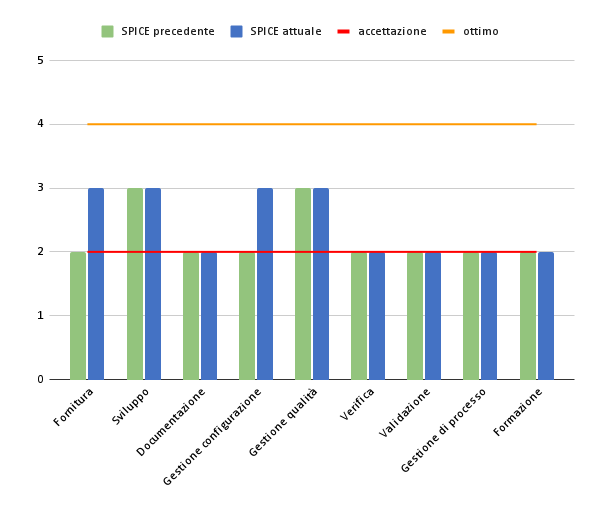
\includegraphics[scale=0.50]{Sezioni/images/vc-spice.png}
    \caption{Validazione e collaudo: MPC01 - SPICE}
\end{figure}

\subsubsection{MPC02 - BCWS}
\begin{figure}[H]
    \centering
    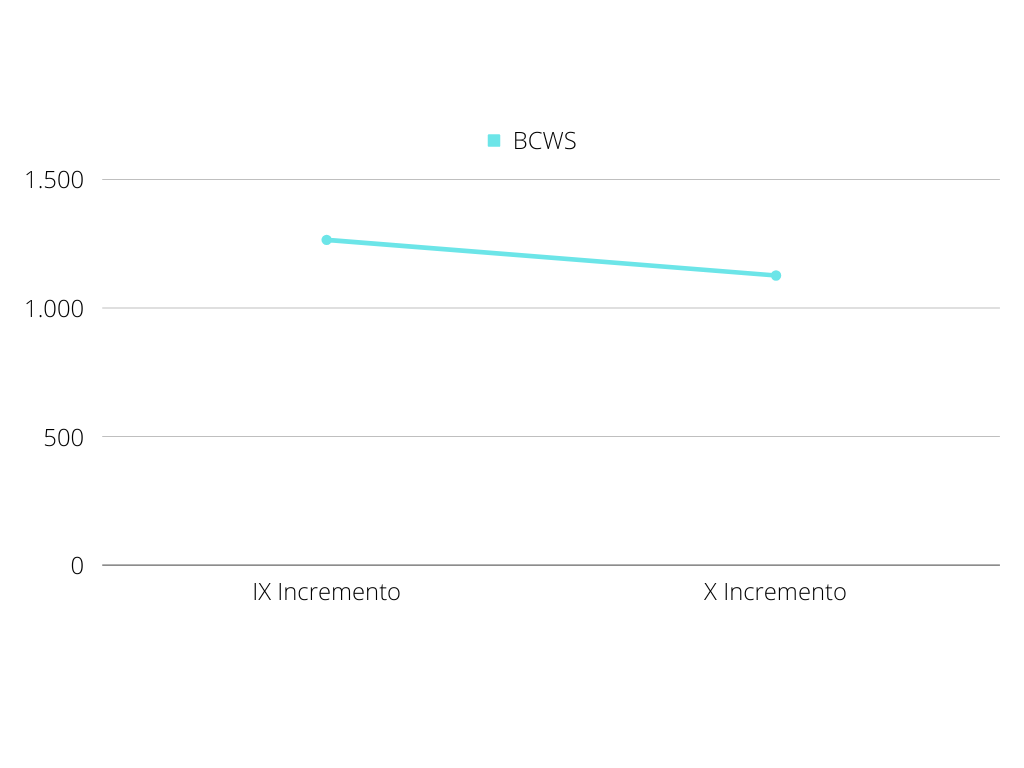
\includegraphics[scale=0.50]{Sezioni/images/vc-BCWS.png}
    \caption{Validazione e collaudo: MPC02 - BCWS}
\end{figure}

\subsubsection{MPC03 - ACWP}
\begin{figure}[H]
    \centering
    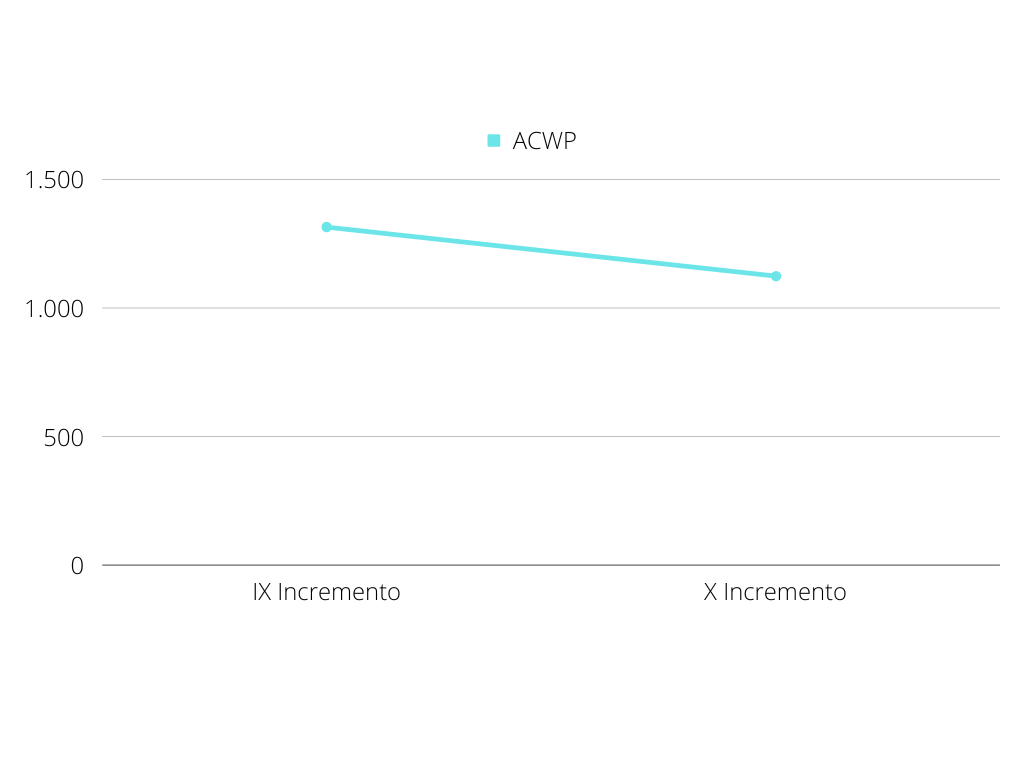
\includegraphics[scale=0.50]{Sezioni/images/vc-ACWP.png}
    \caption{Validazione e collaudo: MPC03 - ACWP}
\end{figure}

\subsubsection{MPC04 - BCWP}
\begin{figure}[H]
    \centering
    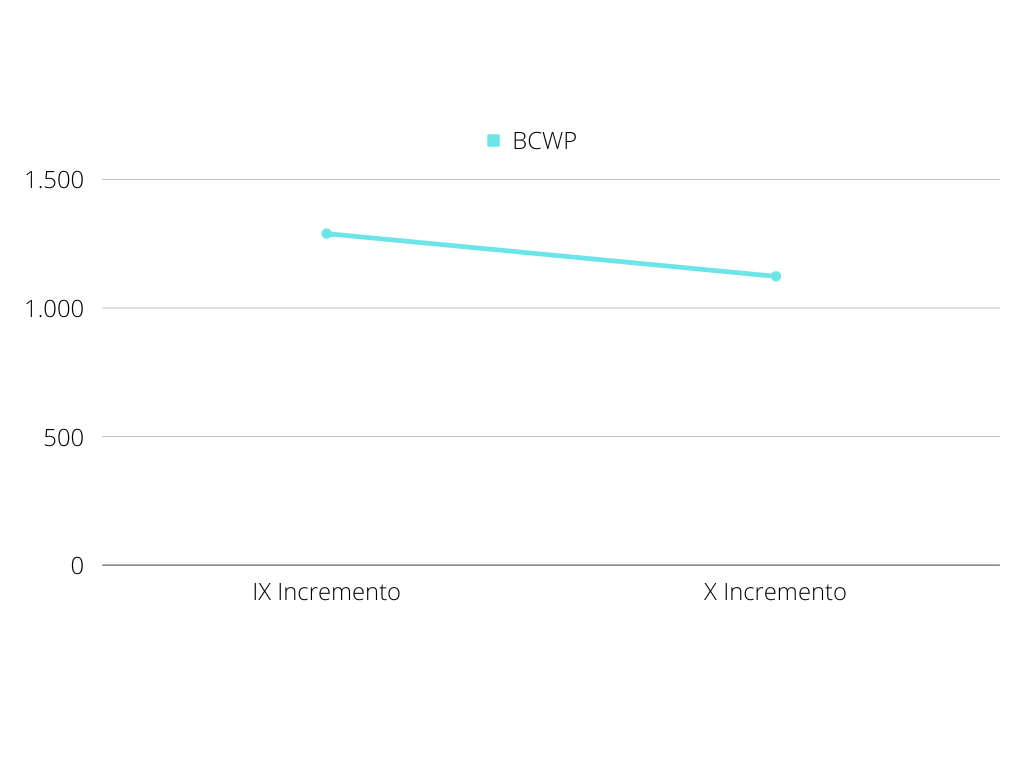
\includegraphics[scale=0.50]{Sezioni/images/vc-BCWP.png}
    \caption{Validazione e collaudo: MPC04 - BCWP}
\end{figure}

\subsubsection{MPC05 - Schedule variance}
La Schedule variance raggiunge un valore ottimo in entrambi gli incrementi.
\begin{figure}[H]
    \centering
    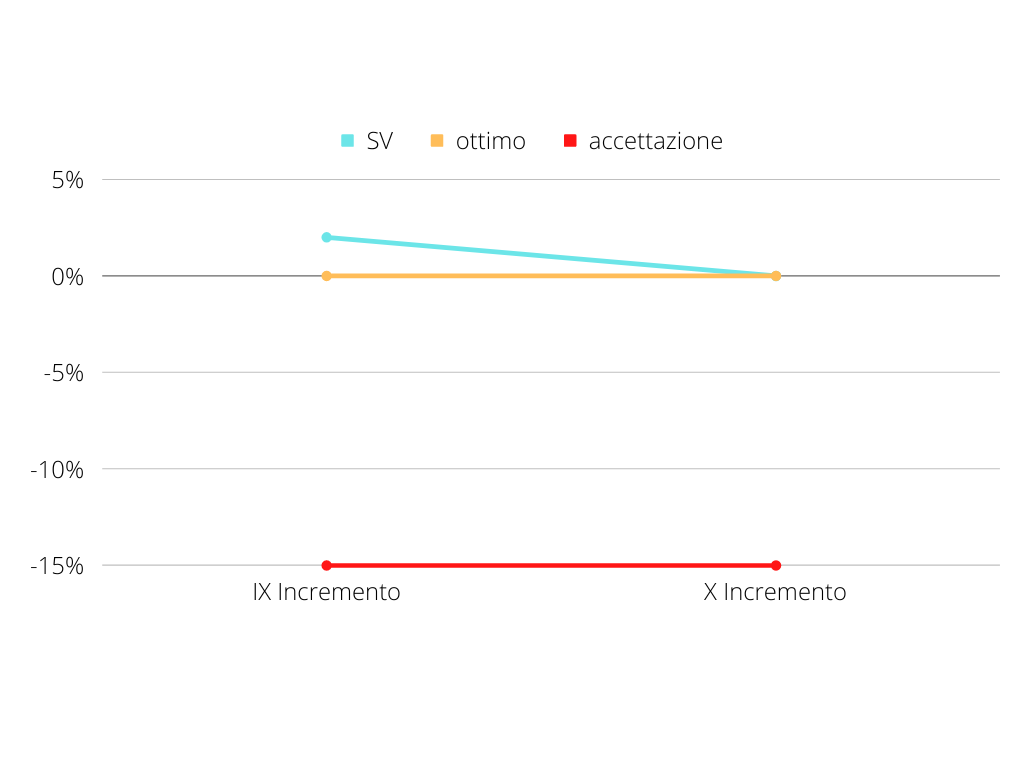
\includegraphics[scale=0.50]{Sezioni/images/vc-SV.png}
    \caption{Validazione e collaudo: MPC05 - SV}
\end{figure}

\subsubsection{MPC06 - Budget variance}
La Budget variance raggiunge un valore accettabile nel IX incremento ed un valore ottimo nel X incremento.
\begin{figure}[H]
    \centering
    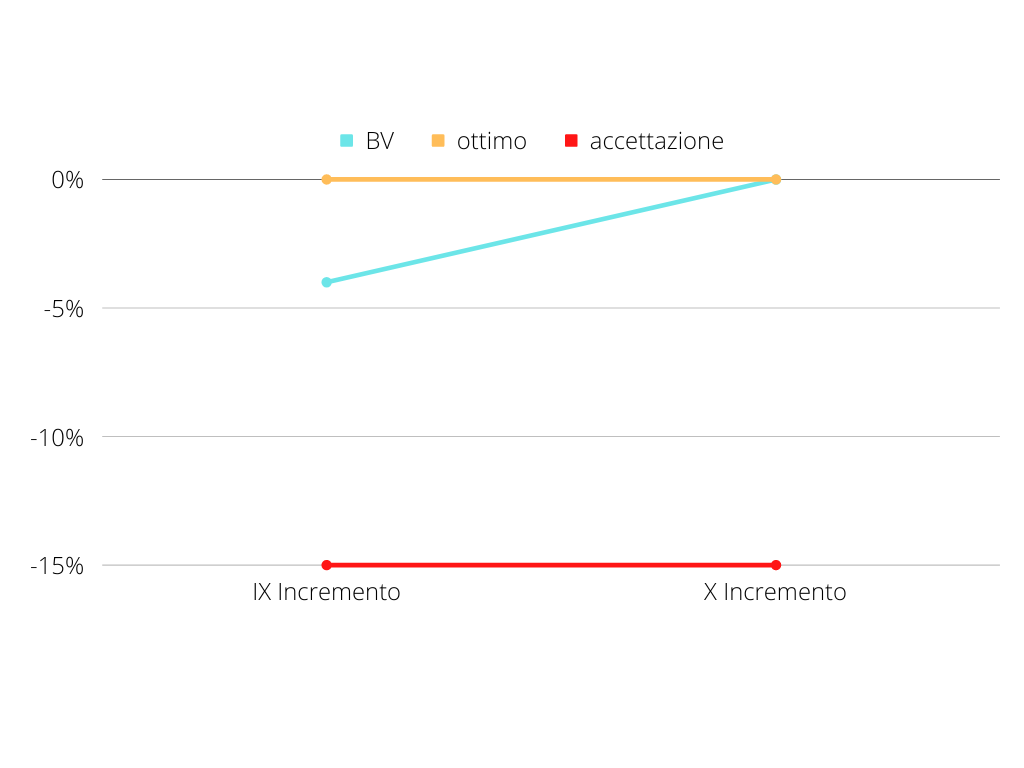
\includegraphics[scale=0.50]{Sezioni/images/vc-BV.png}
    \caption{Validazione e collaudo: MPC06 - BV}
\end{figure}
% \subsection{Periodo di Validazione e collaudo}
\subsubsection{MQP01 - Indice di Gulpease}
Di seguito sono riportati, attraverso l'uso di una tabella e di diagrammi, i valori rilevati al termine dell'ultimo incremento, tutti i documenti hanno raggiunto il vaolore ottimale.
\begin{table}[H]
    \rowcolors{2}{gray!25}{white}
    \rowcolors{2}{gray!25}{white}
        \renewcommand{\arraystretch}{1.5}
        \begin{tabular}{m{0.4\textwidth}<{\centering}  m{0.25\textwidth}<{\centering}  m{0.25\textwidth}<{\centering} }
            \rowcolor{darkblue}
            \textcolor{white}{\textbf{Documento}}& \textcolor{white}{\textbf{Valore}} & \textcolor{white}{\textbf{Esito}}\\ 

            \textit{NormeDiProgetto-v3.0.0} &
            70 &
            Superato \\

            \textit{PianoDiProgetto-v3.0.0} &
            78 &
            Superato \\

            \textit{PianoDiQualifica-v3.0.0} &
            75 &
            Superato \\

            \textit{AnalisiDeiRequisiti-v3.0.0} &
            90 &
            Superato \\
            
            \textit{Glossario-v3.0.0} &
            82 &
            Superato \\
            \textit{SpecificaArchitetturale-v2.0.0} &
            85 &
            Superato \\
            \textit{ManualeUtente-v2.0.0} &
            82 &
            Superato \\

            \textit{VerbaleEsterno-2022.06.07} &
            72 &
            Superato \\
          
            \textit{VerbaleInterno-2022.06.06} &
            75&
            Superato \\
    \end{tabular}
    \caption{Validazione e collaudo: MQP01 - Indice di Gulpease}
\end{table}
\begin{figure}[H]
    \centering
    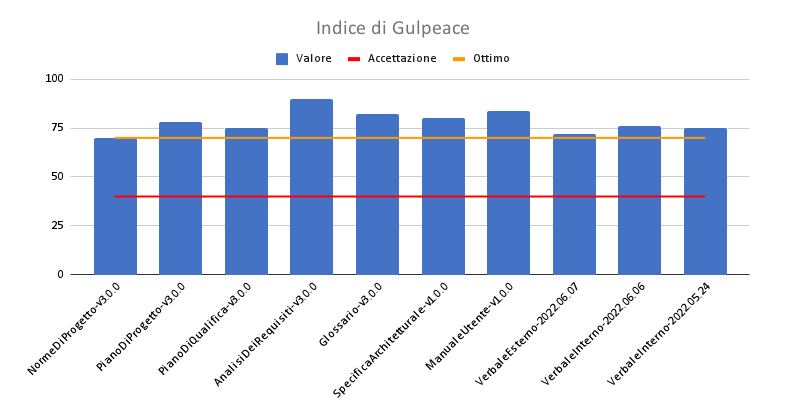
\includegraphics[scale=0.50]{Sezioni/images/last_prodotto/Indice_di_Gulpeace.png}
    \caption{Validazione e collaudo: MPC02 - BCWS}
\end{figure}
\subsubsection{MQP02 - Profondità di una gerarchia}
Siamo riusciti a ridurre la profondità della gerarchia di una classe a 1 durante ultimo incremento nella parte back-end del progetto.
\begin{figure}[H]
    \centering
    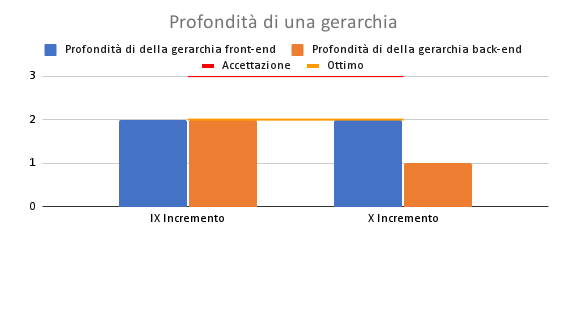
\includegraphics[scale=0.50]{Sezioni/images/last_prodotto/Profondita_di_una_gerarchia.png}
    \caption{Validazione e collaudo: MQP02 - Profondità di una gerarchia}
\end{figure}
\subsubsection{MQP03 - Numero parametri per metodo}
Il numero di parametri per metodo resta invariato comunque il valore è sotto il volaro ottimale.
\begin{figure}[H]
    \centering
    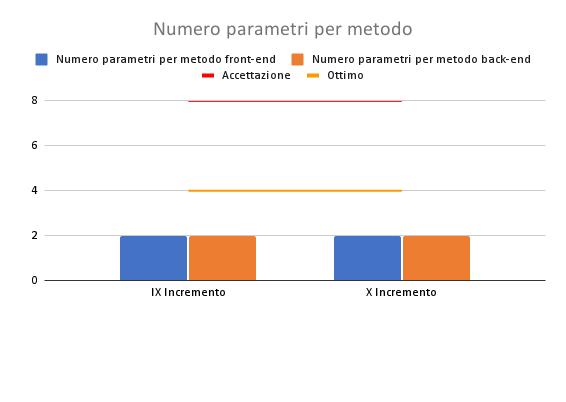
\includegraphics[scale=0.50]{Sezioni/images/last_prodotto/Numero_parametri_per_metodo.png}
    \caption{Validazione e collaudo: MQP03 - Numero parametri per metodo}
\end{figure}
\subsubsection{MQP04 - Code coverage}
Il codecoverage è aumentato durante ultimi incrementi sia nella parte frontend che nella parte back-end, grazie alla miglioria della qualità del codice.
\begin{figure}[H]
    \centering
    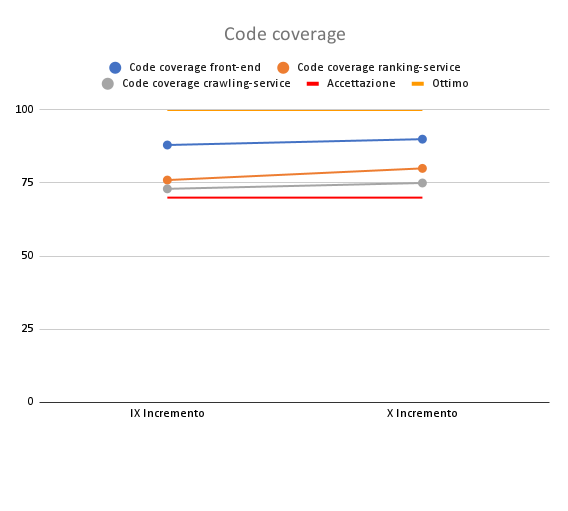
\includegraphics[scale=0.50]{Sezioni/images/last_prodotto/Code_coverage.png}
    \caption{Validazione e collaudo: MQP04 - Code coverage}
\end{figure}
\subsubsection{MQP05 - Percentuale requisiti obbligatori soddisfatti}
Nella fase finale del progetto il gruppo è riuscito a soddisfare tutti requisiti obbligatori.
\begin{figure}[H]
    \centering
    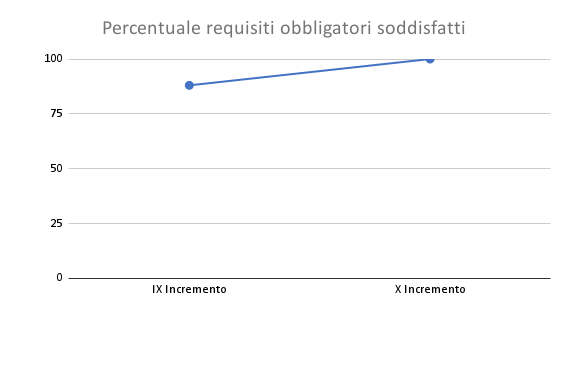
\includegraphics[scale=0.50]{Sezioni/images/last_prodotto/Percentuale_requisiti_obbligatori_soddisfatti.png}
    \caption{Validazione e collaudo: MQP05 - Percentuale requisiti obbligatori soddisfatti}
\end{figure}
\subsubsection{MQP06 - Complessità ciclomatica}
Il gruppo durante ultima fase è riuscito a raggiunge il valore ottimale complessità ciclomatica, grazie all'implementazione della nuova funzionalità.
\begin{figure}[H]
    \centering
    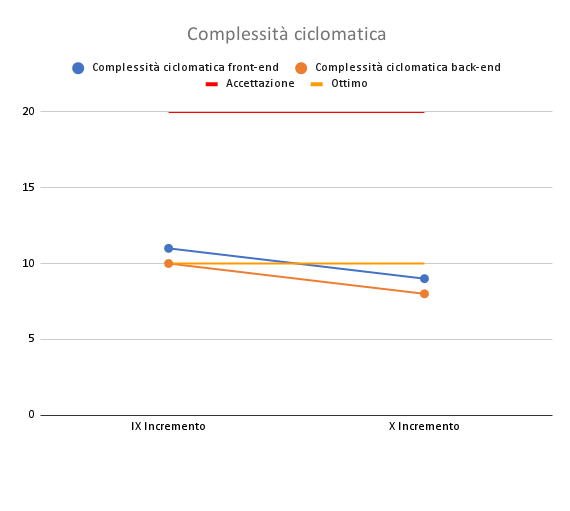
\includegraphics[scale=0.50]{Sezioni/images/last_prodotto/Complessita_ciclomatica.png}
    \caption{Validazione e collaudo: MQP06 - Complessità ciclomatica}
\end{figure}
\subsubsection{MQP07 - Numero di bug}
Rispetto ai precedenti incrementi nelle ultime due fasi del progetto, il gruppo è riuscito ad azzerare il numero di bug.
\begin{figure}[H]
    \centering
    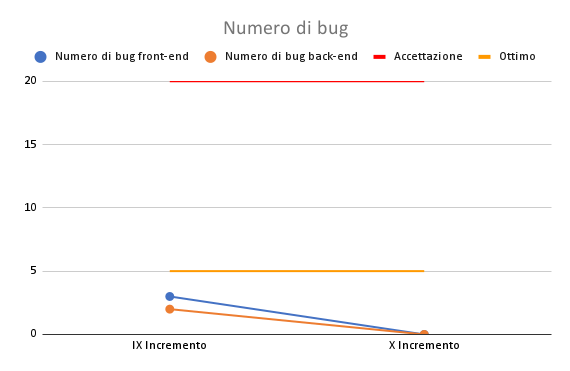
\includegraphics[scale=0.50]{Sezioni/images/last_prodotto/Numero_di_bug.png}
    \caption{Validazione e collaudo: MQP07 - Numero di bug}
\end{figure}
\subsubsection{MQP08 - Numero di Code smell}
Il gruppo durante ultima fase è riuscito a raggiungere il valore ottimale numero di Code smell dopo il collaudo finale.
\begin{figure}[H]
    \centering
    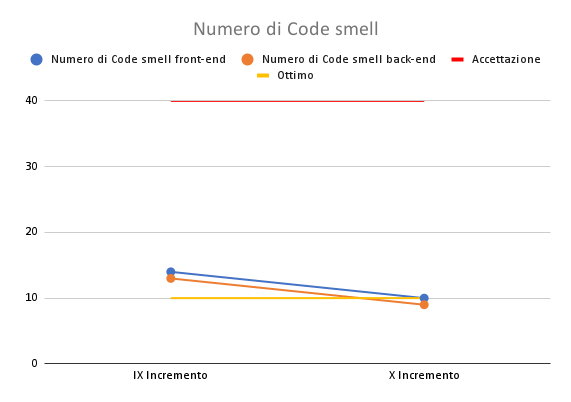
\includegraphics[scale=0.50]{Sezioni/images/last_prodotto/Numero_di_Code_smell.png}
    \caption{Validazione e collaudo: MQP08 - Numero di Code smell}
\end{figure}
\subsubsection{MQP09 - Linee di Commento per Linee di Codice}
Nell'ultimo incremento il progetto ha raggiunto il valore di accettazione richiesto per i linee di commento per linee di codice.
\begin{figure}[H]
    \centering
    \includegraphics[scale=0.50]{Sezioni/images/last_prodotto/Linee_di_Commento_per Linee_di_Codice.png}
    \caption{Validazione e collaudo: MQP09 - Linee di Commento per Linee di Codice}
\end{figure}
\subsubsection{MQP10 - Branch Coverage}
Il branch coverage è aumentato durante ultimi incrementi sia nella parte frontend che nella parte back-end e si avvicina sempre al valore ottimale.
\begin{figure}[H]
    \centering
    \includegraphics[scale=0.50]{Sezioni/images/last_prodotto/Branch_coverage.png}
    \caption{Validazione e collaudo: MQP10 - Branch Coverage}
\end{figure}
\subsubsection{MQP11 - Successo di test}
La successione di test nella parte back-end è arrivato al valore ottimale, per la parte front-end la successione di test è aumentata di 10 percento.
\begin{figure}[H]
    \centering
    \includegraphics[scale=0.50]{Sezioni/images/last_prodotto/Successo_dei_test.png}
    \caption{Validazione e collaudo: MQP11 - Successo di test}
\end{figure}
\subsubsection{MQP12 - Numero di vulnerabilità}
Il gruppo durante ultima fase è riuscito a raggiungere il valore ottimale numero di vulnerabilità rimuovendo tutte le vulnerabilità che aveva il progetto nelle fasi precedenti.
\begin{figure}[H]
    \centering
    \includegraphics[scale=0.50]{Sezioni/images/last_prodotto/Numero_di_vulnerabilita.png}
    \caption{Validazione e collaudo: MQP12 - Numero di vulnerabilità}
\end{figure}

\subsubsection{MTS1 - Test eseguiti in rapporto ai requisiti}
\begin{table}[H]
    \rowcolors{2}{gray!25}{white}
    \renewcommand{\arraystretch}{1.5}
    \begin{tabular}{ m{0.4\textwidth}<{\centering}  m{0.2\textwidth}<{\centering}  m{0.2\textwidth}<{\centering} m{0.2\textwidth}<{\centering} }
        \rowcolor{darkblue}
        \textcolor{white}{\textbf{Incremento}} &\textcolor{white}{\textbf{Valore calcolato}}& \textcolor{white}{\textbf{Valore ottimo}} & \textcolor{white}{\textbf{Valore tollerato}}\\ 
        
        IX Incremento & 
        100\% &
        100\% &
        100\% \\

        X Incremento & 
        100\% &
        100\% &
        100\% \\

    \end{tabular}
    \caption{Validazione e collaudo: MTS1 - Test eseguiti in rapporto ai requisiti}
\end{table}

\subsubsection{MTS2 - Percentuale test passati}
\begin{table}[H]
    \rowcolors{2}{gray!25}{white}
    \renewcommand{\arraystretch}{1.5}
    \begin{tabular}{ m{0.4\textwidth}<{\centering}  m{0.2\textwidth}<{\centering}  m{0.2\textwidth}<{\centering} m{0.2\textwidth}<{\centering} }
        \rowcolor{darkblue}
        \textcolor{white}{\textbf{Incremento}} &\textcolor{white}{\textbf{Valore calcolato}}& \textcolor{white}{\textbf{Valore ottimo}} & \textcolor{white}{\textbf{Valore tollerato}}\\ 
        
        IX Incremento & 
        100\% &
        100\% &
        85\% \\

        X Incremento & 
        100\% &
        100\% &
        85\% \\

    \end{tabular}
    \caption{Validazione e collaudo: MTS2 - Percentuale test passati}
\end{table}